\documentclass[11pt]{article}
\usepackage[margin=0.85in]{geometry}
\usepackage{amsmath, amssymb}
\usepackage{graphicx}
\usepackage{float}
\usepackage{booktabs}
\usepackage[font=small,labelfont=bf]{caption}
\usepackage{xcolor}
\usepackage{enumitem}
\usepackage{hyperref}
\usepackage{multirow}
\usepackage{siunitx}
\hypersetup{colorlinks=true,linkcolor=blue!60!black,urlcolor=blue!60!black}

\title{\Large\textbf{GAD vs Sella vs Hybrid GAD--Newton}\\[4pt]
\large Aggregated TS-finder benchmark on Transition1x test split\\[2pt]
\normalsize 2026-05-16. $n=287$ samples per (method, noise). Headline + convergence-criterion sensitivity.}
\author{}
\date{}

\begin{document}
\maketitle
\thispagestyle{empty}

% =================================================================
\section*{TL;DR}
% =================================================================

Three families, six noise levels (10--200 pm), starting condition: noised
true T1x TS. Best of each family:

\begin{center}\small\fbox{\parbox{0.95\textwidth}{
\textbf{Sella cartesian Eckart untuned Hess.Freq.=1} wins TS conv $\le$50 pm (92.7\% @ 10 pm).
\textbf{Plain GAD dt=0.005} wins IRC TOPO at $\ge$100 pm (+11.9 pp over Sella at 150 pm; +21.3 pp at 200 pm).
\textbf{Hybrid damped Eckart eig-switch tr=0.05} wins \emph{wall-time per converged TS}
at every noise (1.4--3.0$\times$ vs Sella; 4.1--4.5$\times$ vs plain GAD),
and produces \emph{geometrically tighter} TSs than either baseline at high noise
(p95 RMSD-to-known-TS at 200 pm: hybrid 0.11 Å vs Sella 0.84 Å vs plain GAD 0.46 Å).
}}
\end{center}

\paragraph{Sella naming convention (used throughout).}
The project's historical names (\texttt{libdef}, \texttt{default}, \texttt{internal})
were inconsistent. This report uses a three-axis name:

\begin{center}\footnotesize
\textbf{Sella \{cartesian | internal\} \{Eckart\}? \{tuned | untuned\} Hess.Freq.=N}
\end{center}

\begin{itemize}[leftmargin=1.5em, itemsep=0.05em]
\item \textbf{coords}: \texttt{cartesian} or \texttt{internal} (only Cartesian needs Eckart projection)
\item \textbf{Eckart}: present only if Eckart projection is applied
\item \textbf{tuned}: trust-radius hyperparameters $(\delta_0,\gamma)$ tuned from Sella's library defaults.
  \texttt{tuned}: $\delta_0{=}0.048$, $\gamma{=}0$ (this project's choice); \texttt{untuned}: $\delta_0{=}0.1$, $\gamma{=}0.4$ (Sella library defaults)
\item \textbf{Hess.Freq.=N}: Hessian recomputed every $N$ steps. Sella library default is 3; our project canonical is 1.
\end{itemize}

\begin{center}\footnotesize
\textbf{Historical $\to$ new name map}\\[0.3em]
\begin{tabular}{l|l}
\toprule
\textbf{Old name} & \textbf{New name (this report)} \\
\midrule
\texttt{Sella libdef} (cart+Eckart, $\delta_0{=}0.1$, $\gamma{=}0.4$, d=1) & Sella cartesian Eckart untuned Hess.Freq.=1 \\
\texttt{Sella default} (cart no-Eckart, $\delta_0{=}0.048$, $\gamma{=}0$, d=1) & Sella cartesian tuned Hess.Freq.=1 \\
\texttt{Sella internal} (internal coords, $\delta_0{=}0.048$, $\gamma{=}0$, d=1) & Sella internal tuned Hess.Freq.=1 \\
\texttt{Sella libdef Hess-freq d=3} & Sella cartesian Eckart untuned Hess.Freq.=3 \\
\bottomrule
\end{tabular}
\end{center}

\paragraph{Recommendation.}
\begin{center}\small
\begin{tabular}{p{0.30\textwidth}|p{0.42\textwidth}|p{0.22\textwidth}}
\toprule
\textbf{Goal} & \textbf{Use} & \textbf{Why} \\
\midrule
Fastest TS finder, any noise & Hybrid damped Eckart eig-switch tr=0.05 & 1.4--3$\times$ vs Sella \\
Highest IRC TOPO at $\ge$100 pm & Plain GAD dt=0.005 & Right-basin failures \\
Tightest geometry at high noise & Hybrid damped Eckart eig-switch tr=0.05 & 7.7$\times$ tighter p95 \\
Low-noise TS conv ($\le$50 pm) & Sella cartesian Eckart untuned Hess.Freq.=1 & 92.7\% @ 10 pm \\
\bottomrule
\end{tabular}
\end{center}

\clearpage
% =================================================================
\section{Headline figure 1 — best-of-family across TS noise (noised true TS)}
% =================================================================

The starting condition for this sweep is the \textbf{noised true T1x TS}
(Gaussian perturbation of the labelled saddle geometry). Six noise levels,
identical sample set, project-canonical convergence criterion
$n_\text{neg}{=}1 \wedge F_\text{max}<0.01$ eV/Å.

\begin{figure}[H]
\centering
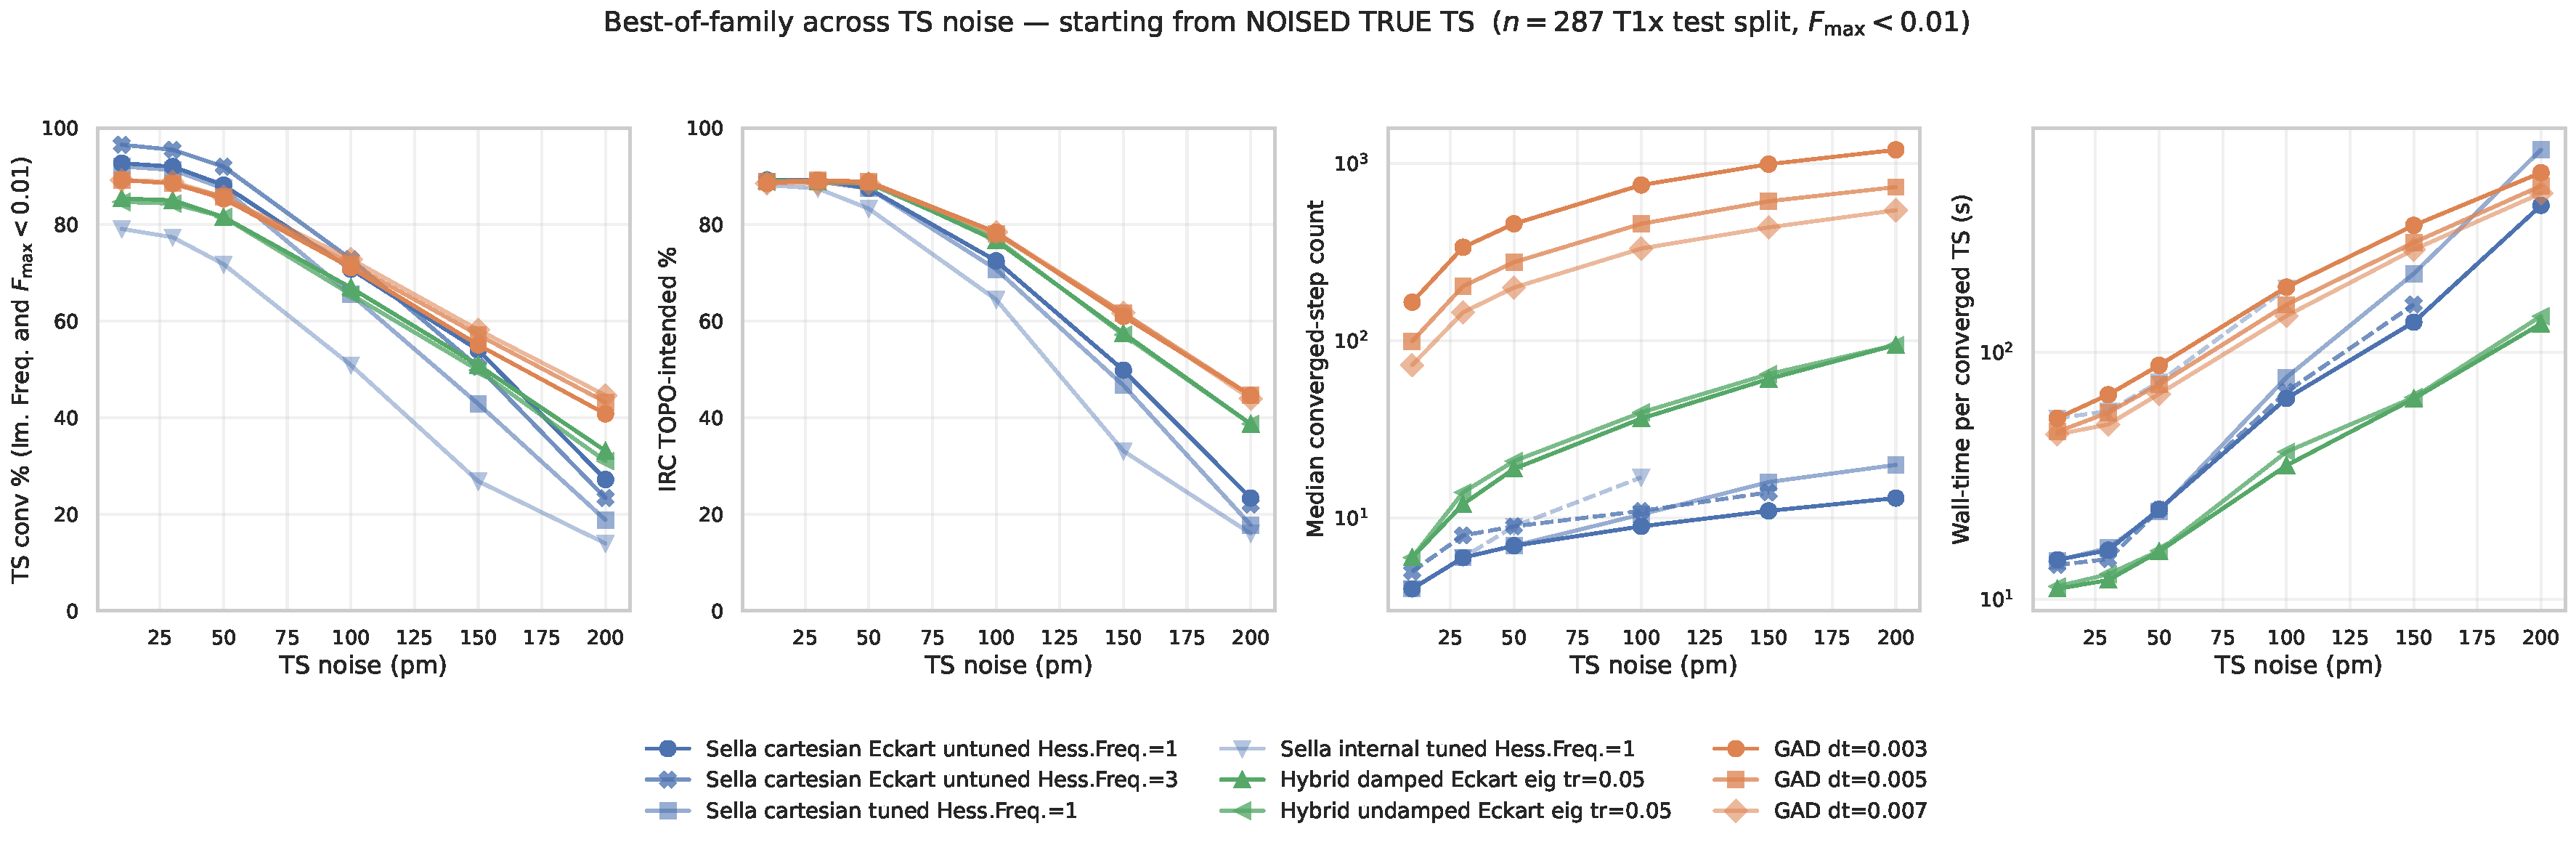
\includegraphics[width=\textwidth]{figures_2026_05_16/fig_main_4axis.pdf}
\caption{\textbf{Best-of-family, four diagnostic axes.} TS conv, IRC TOPO,
median converged-step count, wall-time per converged TS, all as a function
of noise level. Each family contributes its strongest configs as separate
lines. The Hess.Freq.=3 variant is now available across 10--200 pm (200 pm
from pooled main + safety-net partitions, $n=53$);
Sella internal goes 10--100 pm only. All others span the full 10--200 pm grid.
Source: \texttt{master\_2026\_05\_11.csv}.}
\end{figure}

\paragraph{Per-noise tables.} All numbers from
\texttt{analysis\_2026\_04\_29/master\_2026\_05\_11.csv}. Bold = best in row.
$^p$ = partial: extracted from SLURM log after timeout (biased toward smaller
molecules; see Section~\ref{sec:sources}). Subscripts on $^{p}$ indicate the
sample count when known and the source is pooled (main + safety-net
partitions), so the bias is reduced relative to log-only extraction.

\begin{center}\footnotesize
\textbf{Table 1 — TS conv \%} (Im. Freq. and $F_\mathrm{max}<0.01$, $n=287$)\\[0.3em]
\begin{tabular}{l|cccccc}
\toprule
\textbf{method} & \textbf{10 pm} & \textbf{30 pm} & \textbf{50 pm} & \textbf{100 pm} & \textbf{150 pm} & \textbf{200 pm} \\
\midrule
GAD dt=0.003                                & 89.2 & 88.5 & 85.4 & 71.1 & 55.1 & 40.8 \\
GAD dt=0.005                                & 89.2 & 88.5 & 85.7 & 71.8 & 57.1 & 43.2 \\
GAD dt=0.007                                & 89.2 & 88.9 & 85.7 & 72.8 & 58.2 & \textbf{44.6} \\
\midrule
Sella cartesian tuned Hess.Freq.=1          & 92.0 & 91.3 & 87.5 & 65.5 & 42.9 & 18.8 \\
Sella cartesian Eckart untuned Hess.Freq.=1 & 92.7 & 92.0 & 88.2 & 70.7 & 54.0 & 27.2 \\
Sella internal tuned Hess.Freq.=1           & 79.1 & 77.4 & 71.8 & 50.9 & 26.8 & 13.9 \\
Sella cartesian Eckart untuned Hess.Freq.=3 & \textbf{96.5} & \textbf{95.5} & \textbf{92.0} & 72.8 & 50.5 & 23.3 \\
\midrule
Hybrid damped Eckart eig tr=0.05            & 85.4 & 85.0 & 81.5 & 66.9 & 50.9 & 33.1 \\
Hybrid undamped Eckart eig tr=0.05          & 84.7 & 84.3 & 81.5 & 65.5 & 49.8 & 31.0 \\
\bottomrule
\end{tabular}
\end{center}

\begin{center}\footnotesize
\textbf{Table 2 — IRC TOPO-intended \%} (forward+backward Sella IRC + graph-match to T1x reactant/product, $n=287$)\\[0.3em]
\begin{tabular}{l|cccccc}
\toprule
\textbf{method} & \textbf{10 pm} & \textbf{30 pm} & \textbf{50 pm} & \textbf{100 pm} & \textbf{150 pm} & \textbf{200 pm} \\
\midrule
GAD dt=0.003                                & 88.5 & \textbf{89.2} & 88.9 & 78.4 & 61.0 & 44.6 \\
GAD dt=0.005                                & 88.9 & \textbf{89.2} & 88.9 & 78.0 & 61.7 & \textbf{44.6} \\
GAD dt=0.007                                & 88.5 & 88.5 & 88.5 & \textbf{78.4} & \textbf{61.7} & 43.9 \\
\midrule
Sella cartesian tuned Hess.Freq.=1          & 88.9 & 88.9 & 87.5 & 70.7 & 46.7 & 17.8 \\
Sella cartesian Eckart untuned Hess.Freq.=1 & \textbf{89.2} & \textbf{89.2} & 87.5 & 72.5 & 49.8 & 23.3 \\
Sella internal tuned Hess.Freq.=1           & 88.2 & 87.5 & 83.3 & 64.5 & 33.1 & 16.0 \\
Sella cartesian Eckart untuned Hess.Freq.=3 & 88.5 & 88.9 & 87.1 & 70.4 & 45.3 & 22.0 \\
\midrule
Hybrid damped Eckart eig tr=0.05            & \textbf{89.2} & 88.9 & 88.9 & 76.7 & 57.5 & 38.7 \\
Hybrid undamped Eckart eig tr=0.05          & 88.9 & 88.9 & 88.5 & 77.0 & 57.1 & 38.7 \\
\bottomrule
\end{tabular}
\end{center}

\clearpage
% =================================================================
\section{Convergence-criterion families: which $F_\mathrm{max}$ threshold?}
\label{sec:thresholds}
% =================================================================

The figure-1 4-axis comparison uses $F_\mathrm{max}<0.01$ as the convergence
threshold. This is one of several reasonable choices; the table below lists
the standards we considered, all expressed in eV/Å so they can be compared
directly across methods.

\begin{center}\small
\textbf{Convergence-criterion candidates (force component on a single atom).}\\[0.4em]
\begin{tabular}{l|c|c|p{0.36\textwidth}}
\toprule
\textbf{Standard} & \textbf{Threshold (eV/Å)} & \textbf{In other units} & \textbf{Note} \\
\midrule
ASE \texttt{Optimizer.run(fmax=...)} default      & 0.05    & 0.05 eV/Å              & Used by all ASE-inherited optimizers including Sella's parent class \\
Gaussian "Loose"                                   & $\sim$0.05  & --                 & Comparable to ASE default \\
\textbf{Gaussian "Normal" (Max Force)}             & \textbf{0.0231} & $4.50\times10^{-4}~E_h/a_0$ & Standard quantum-chemistry default; one of four Gaussian criteria \\
Gaussian "Normal" (RMS Force)                      & 0.0154  & $3.00\times10^{-4}~E_h/a_0$ & Companion to Max Force; tested simultaneously by Gaussian \\
\textbf{This project (canonical)}                  & \textbf{0.01}   & --                  & Default for new sweeps; balanced strict-but-reachable \\
Tight                                              & 0.005   & --                  & Reached only by Newton steps; pure GAD plateaus near 0.01 \\
Sella README recommendation                        & \textbf{0.001}  & --                  & Cited in the Sella README as a fully-converged TS; not reachable for any method we tested within 2000 steps \\
\bottomrule
\end{tabular}
\end{center}

\paragraph{Gaussian "Normal" full criterion set (for the record).}
Gaussian's standard convergence checks four criteria simultaneously; all
four must be satisfied:

\begin{center}\footnotesize
\begin{tabular}{l|r|r}
\toprule
\textbf{Criterion} & \textbf{Threshold (a.u.)} & \textbf{Converted (eV/Å or Å)} \\
\midrule
Maximum Force ($F_\text{max}$)                     & $4.50\times10^{-4}~E_h/a_0$ & \SI{0.02314}{eV/\angstrom} \\
RMS Force ($F_\text{RMS}$)                         & $3.00\times10^{-4}~E_h/a_0$ & \SI{0.01543}{eV/\angstrom} \\
Maximum Displacement ($\Delta q_\text{max}$)       & $1.80\times10^{-3}~a_0$     & \SI{9.525e-4}{\angstrom}   \\
RMS Displacement ($\Delta q_\text{RMS}$)           & $1.20\times10^{-3}~a_0$     & \SI{6.350e-4}{\angstrom}   \\
\bottomrule
\end{tabular}
\end{center}

Conversions: $1\,E_h/a_0 = 51.4220675$~eV/Å, $1\,a_0 = 0.5291772105$~Å.

\paragraph{Threshold-sweep results.} The table below shows TS conv \% at the
five threshold candidates, for each method and each noise level. Sella tracks
the threshold smoothly (because its Newton step pushes force down); plain
GAD \emph{collapses} below 0.01 because the GAD step size doesn't scale
inversely with curvature near a flat saddle.

\begin{center}\footnotesize
\textbf{Table 3 — TS conv \% across $F_\mathrm{max}$ thresholds} (starting from noised TS, $n=287$).\\
\textit{0.05}: ASE default;\quad\textit{0.023}: Gaussian Normal;\quad\textit{0.01}: project canonical;\quad\textit{0.005}: tight;\quad\textit{0.001}: Sella README.\\[0.3em]
\begin{tabular}{l|c|ccccc}
\toprule
\textbf{method} & \textbf{noise} & \textbf{0.05} & \textbf{0.023} & \textbf{0.01} & \textbf{0.005} & \textbf{0.001} \\
\midrule
\multirow{6}{*}{GAD dt=0.007}
 & 10  & 98.3 & 95.1 & 89.2 & 0.0  & 0.0 \\
 & 30  & 97.9 & 95.5 & 88.9 & 0.0  & 0.0 \\
 & 50  & 94.8 & 91.6 & 85.7 & 0.0  & 0.0 \\
 & 100 & 82.6 & 77.7 & 72.8 & 0.0  & 0.0 \\
 & 150 & 71.4 & 64.1 & 58.2 & 0.0  & 0.0 \\
 & 200 & 68.3 & 56.4 & 44.6 & 0.0  & 0.0 \\
\midrule
\multirow{6}{*}{Hybrid damped Eckart eig tr=0.05}
 & 10  & 97.2 & 93.0 & 85.4 & 7.3  & 0.0 \\
 & 30  & 96.9 & 92.3 & 85.0 & 9.4  & 0.0 \\
 & 50  & 93.0 & 88.5 & 81.5 & 10.8 & 0.0 \\
 & 100 & 78.0 & 73.5 & 66.9 & 9.1  & 0.0 \\
 & 150 & 59.6 & 55.7 & 50.9 & 7.0  & 0.0 \\
 & 200 & 44.9 & 37.6 & 33.1 & 6.6  & 0.0 \\
\midrule
\multirow{6}{*}{Sella cartesian Eckart untuned Hess.Freq.=1}
 & 10  & 98.6 & 97.9 & 92.7 & 33.8 & 0.0 \\
 & 30  & 98.3 & 97.6 & 92.0 & 32.1 & 0.0 \\
 & 50  & 95.1 & 93.7 & 88.2 & 32.4 & 0.0 \\
 & 100 & 83.3 & 77.7 & 70.7 & 24.7 & 0.0 \\
 & 150 & 66.2 & 59.9 & 54.0 & 15.3 & 0.0 \\
 & 200 & 46.0 & 39.0 & 27.2 & 7.0  & 0.0 \\
\bottomrule
\end{tabular}
\end{center}

\begin{center}\footnotesize
\textbf{Comprehensive Fmax Table — TS conv \% across thresholds, methods, noise levels} ($n=287$ canonical, except where noted).\\[0.4em]
All methods use the noised-true-TS starting condition. Bold values per (threshold, noise) cell.
\end{center}

\begin{center}\footnotesize
\textbf{$F_\mathrm{max}<0.05$} (ASE default)\\[0.3em]
\begin{tabular}{l|cccccc}
\toprule
\textbf{method} & \textbf{10~pm} & \textbf{30~pm} & \textbf{50~pm} & \textbf{100~pm} & \textbf{150~pm} & \textbf{200~pm} \\
\midrule
GAD dt=0.003                   & \textbf{98.6} & \textbf{98.3} & \textbf{95.1} & 82.9 & \textbf{71.8} & 62.7 \\
GAD dt=0.005                   & 98.3 & 97.9 & 94.8 & 82.6 & 71.1 & 63.1 \\
GAD dt=0.007                   & 98.3 & 97.9 & 94.8 & 82.6 & 71.4 & \textbf{68.3} \\
\midrule
S cart tuned d=1               & \textbf{98.6} & 97.9 & 94.4 & 78.0 & 53.7 & 27.9 \\
S cart+Eck untuned d=1         & \textbf{98.6} & \textbf{98.3} & \textbf{95.1} & \textbf{83.3} & 66.2 & 46.0 \\
S internal tuned d=1           & 94.4 & 90.6 & 84.7 & 63.8 & 37.3 & 20.9 \\
S cart+Eck untuned d=3         & \textbf{98.6} & 97.6 & 94.8 & 81.5 & 58.2 & 39.7 \\
\midrule
Hybrid damped                  & 97.2 & 96.9 & 93.0 & 78.0 & 59.6 & 44.9 \\
Hybrid undamped                & 96.5 & 96.2 & 92.7 & 76.7 & 59.6 & 43.9 \\
\bottomrule
\end{tabular}
\end{center}

\begin{center}\footnotesize
\textbf{$F_\mathrm{max}<0.023$} (Gaussian)\\[0.3em]
\begin{tabular}{l|cccccc}
\toprule
\textbf{method} & \textbf{10~pm} & \textbf{30~pm} & \textbf{50~pm} & \textbf{100~pm} & \textbf{150~pm} & \textbf{200~pm} \\
\midrule
GAD dt=0.003                   & 95.5 & 95.1 & 91.6 & 77.4 & 63.1 & 52.3 \\
GAD dt=0.005                   & 95.8 & 95.1 & 91.3 & \textbf{78.0} & 63.8 & 53.7 \\
GAD dt=0.007                   & 95.1 & 95.5 & 91.6 & 77.7 & \textbf{64.1} & \textbf{56.4} \\
\midrule
S cart tuned d=1               & \textbf{97.9} & \textbf{97.6} & 93.0 & 71.8 & 48.4 & 24.7 \\
S cart+Eck untuned d=1         & \textbf{97.9} & \textbf{97.6} & \textbf{93.7} & 77.7 & 59.9 & 39.0 \\
S internal tuned d=1           & 89.5 & 86.1 & 79.1 & 57.5 & 32.4 & 18.1 \\
S cart+Eck untuned d=3         & \textbf{97.9} & 96.9 & 93.4 & 74.6 & 53.7 & 34.5 \\
\midrule
Hybrid damped                  & 93.0 & 92.3 & 88.5 & 73.5 & 55.7 & 37.6 \\
Hybrid undamped                & 93.0 & 92.3 & 88.2 & 71.4 & 54.7 & 37.3 \\
\bottomrule
\end{tabular}
\end{center}

\begin{center}\footnotesize
\textbf{$F_\mathrm{max}<0.01$} (project canonical)\\[0.3em]
\begin{tabular}{l|cccccc}
\toprule
\textbf{method} & \textbf{10~pm} & \textbf{30~pm} & \textbf{50~pm} & \textbf{100~pm} & \textbf{150~pm} & \textbf{200~pm} \\
\midrule
GAD dt=0.003                   & 89.2 & 88.5 & 85.4 & 71.1 & 55.1 & 40.8 \\
GAD dt=0.005                   & 89.2 & 88.5 & 85.7 & 71.8 & 57.1 & 43.2 \\
GAD dt=0.007                   & 89.2 & 88.9 & 85.7 & \textbf{72.8} & \textbf{58.2} & \textbf{44.6} \\
\midrule
S cart tuned d=1               & 92.0 & 91.3 & 87.5 & 65.5 & 42.9 & 18.8 \\
S cart+Eck untuned d=1         & \textbf{92.7} & \textbf{92.0} & \textbf{88.2} & 70.7 & 54.0 & 27.2 \\
S internal tuned d=1           & 79.1 & 77.4 & 71.8 & 50.9 & 26.8 & 13.9 \\
S cart+Eck untuned d=3         & 91.3 & 90.2 & \textbf{88.2} & 67.9 & 48.1 & 23.3 \\
\midrule
Hybrid damped                  & 85.4 & 85.0 & 81.5 & 66.9 & 50.9 & 33.1 \\
Hybrid undamped                & 84.7 & 84.3 & 81.5 & 65.5 & 49.8 & 31.0 \\
\bottomrule
\end{tabular}
\end{center}

\begin{center}\footnotesize
\textbf{$F_\mathrm{max}<0.005$} (tight)\\[0.3em]
\begin{tabular}{l|cccccc}
\toprule
\textbf{method} & \textbf{10~pm} & \textbf{30~pm} & \textbf{50~pm} & \textbf{100~pm} & \textbf{150~pm} & \textbf{200~pm} \\
\midrule
GAD dt=0.003                   & 0.0 & 0.0 & 0.0 & 0.0 & 0.0 & 0.0 \\
GAD dt=0.005                   & 0.0 & 0.0 & 0.0 & 0.0 & 0.0 & 0.0 \\
GAD dt=0.007                   & 0.0 & 0.0 & 0.0 & 0.0 & 0.0 & 0.0 \\
\midrule
S cart tuned d=1               & \textbf{35.9} & \textbf{33.1} & \textbf{34.1} & 22.3 & \textbf{15.7} & 5.6 \\
S cart+Eck untuned d=1         & 33.8 & 32.1 & 32.4 & 24.7 & 15.3 & \textbf{7.0} \\
S internal tuned d=1           & 25.4 & 25.1 & 27.9 & 16.0 & 9.4 & 4.2 \\
S cart+Eck untuned d=3         & 33.4 & 31.7 & 32.1 & \textbf{25.8} & 15.0 & \textbf{7.0} \\
\midrule
Hybrid damped                  & 7.3 & 9.4 & 10.8 & 9.1 & 7.0 & 6.6 \\
Hybrid undamped                & 8.7 & 6.6 & 8.7 & 3.8 & 4.2 & 1.4 \\
\bottomrule
\end{tabular}
\end{center}

\begin{center}\footnotesize
\textbf{$F_\mathrm{max}<0.001$} (Sella README)\\[0.3em]
\begin{tabular}{l|cccccc}
\toprule
\textbf{method} & \textbf{10~pm} & \textbf{30~pm} & \textbf{50~pm} & \textbf{100~pm} & \textbf{150~pm} & \textbf{200~pm} \\
\midrule
GAD dt=0.003                   & \textbf{0.0} & 0.0 & \textbf{0.0} & \textbf{0.0} & \textbf{0.0} & \textbf{0.0} \\
GAD dt=0.005                   & \textbf{0.0} & 0.0 & \textbf{0.0} & \textbf{0.0} & \textbf{0.0} & \textbf{0.0} \\
GAD dt=0.007                   & \textbf{0.0} & 0.0 & \textbf{0.0} & \textbf{0.0} & \textbf{0.0} & \textbf{0.0} \\
\midrule
S cart tuned d=1               & \textbf{0.0} & 0.0 & \textbf{0.0} & \textbf{0.0} & \textbf{0.0} & \textbf{0.0} \\
S cart+Eck untuned d=1         & \textbf{0.0} & 0.0 & \textbf{0.0} & \textbf{0.0} & \textbf{0.0} & \textbf{0.0} \\
S internal tuned d=1           & \textbf{0.0} & 0.0 & \textbf{0.0} & \textbf{0.0} & \textbf{0.0} & \textbf{0.0} \\
S cart+Eck untuned d=3         & \textbf{0.0} & \textbf{0.3} & \textbf{0.0} & \textbf{0.0} & \textbf{0.0} & \textbf{0.0} \\
\midrule
Hybrid damped                  & \textbf{0.0} & 0.0 & \textbf{0.0} & \textbf{0.0} & \textbf{0.0} & \textbf{0.0} \\
Hybrid undamped                & \textbf{0.0} & 0.0 & \textbf{0.0} & \textbf{0.0} & \textbf{0.0} & \textbf{0.0} \\
\bottomrule
\end{tabular}
\end{center}

Numeric source: \texttt{analysis\_2026\_04\_29/threshold\_sweep\_2026\_05\_16.csv}.

\subsection{Headline figure under each threshold (swappable for the paper)}

The five panels below are the same 4-axis figure-1, evaluated under each
threshold. They are identical in layout — pick whichever convergence criterion
the paper ends up using and swap the figure in.

\begin{figure}[H]
\centering
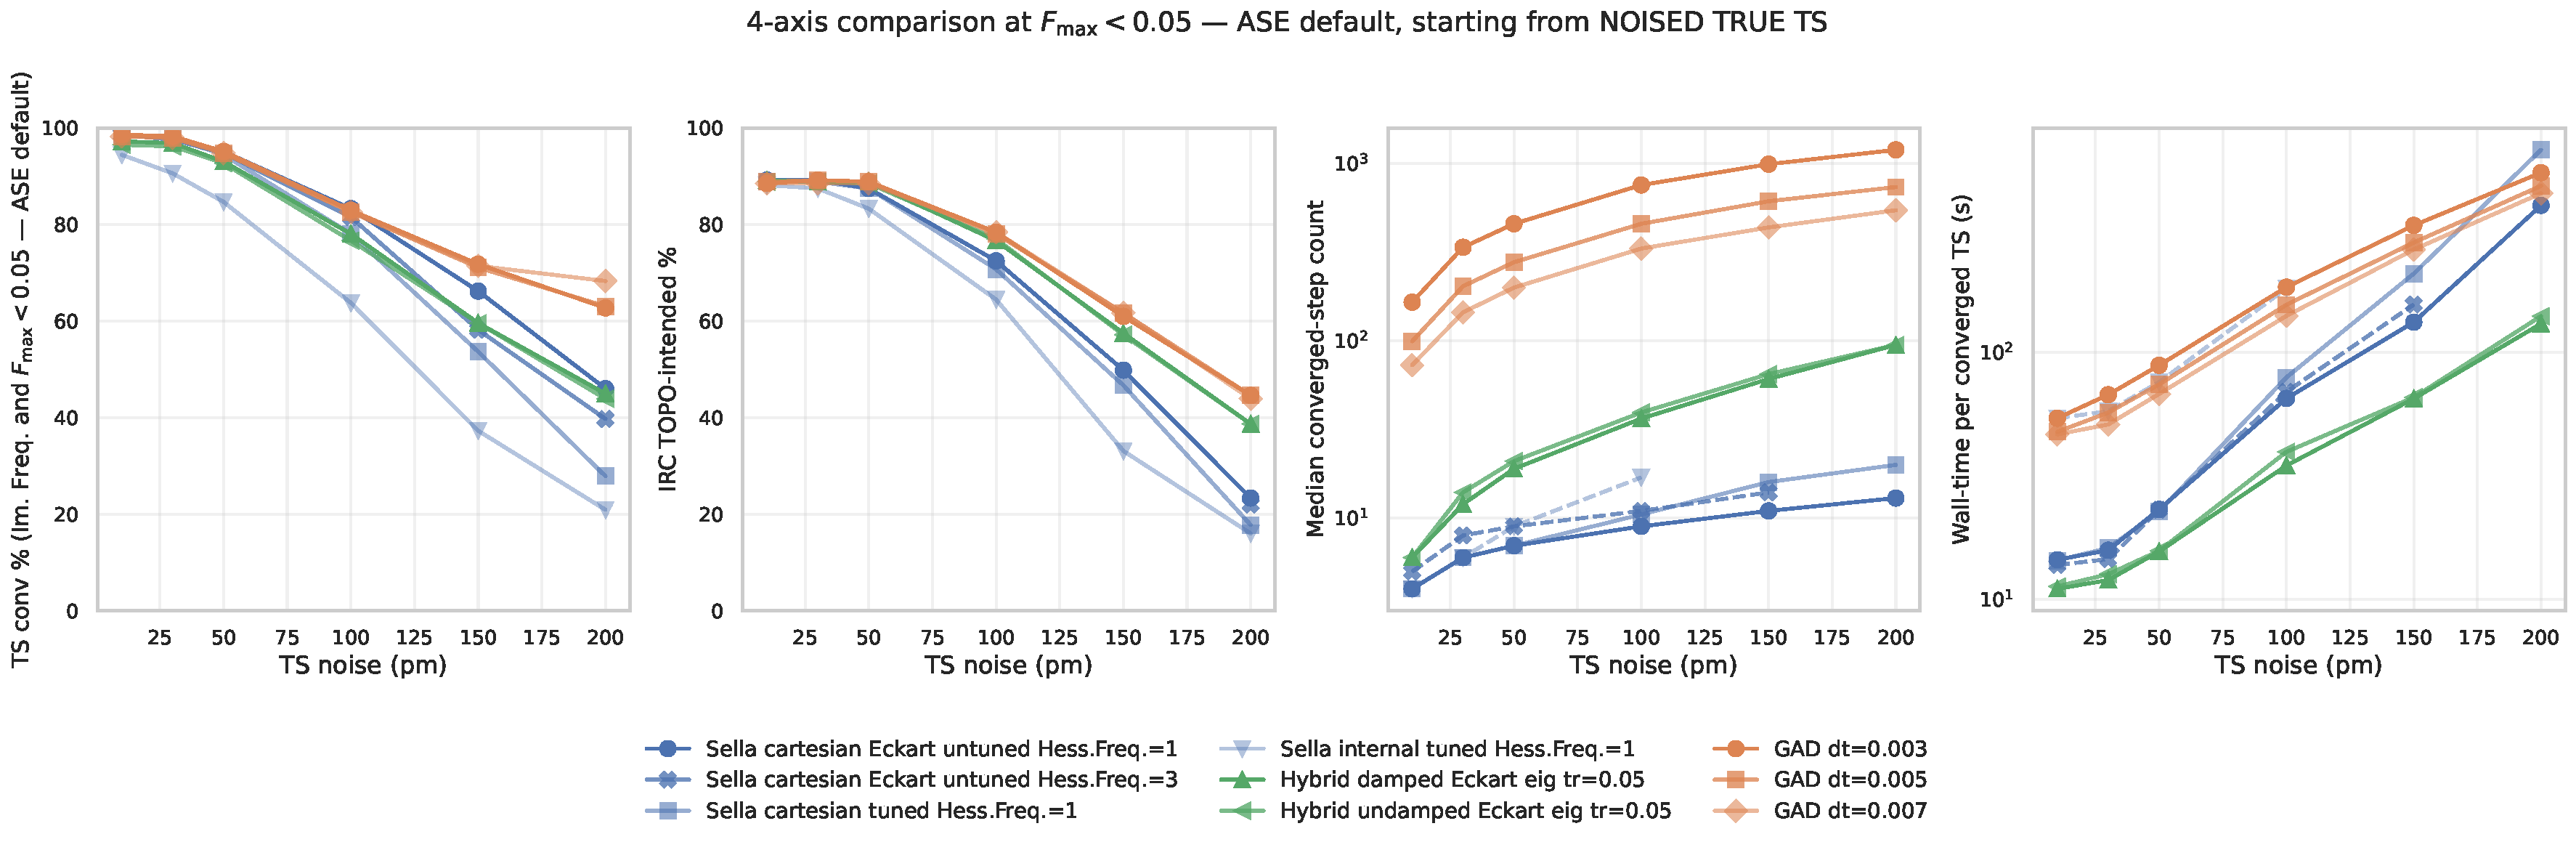
\includegraphics[width=\textwidth]{figures_2026_05_16/fig_main_4axis_fmax0p05.pdf}
\caption{\textbf{4-axis @ $F_\mathrm{max}<0.05$ (ASE default).} GAD,
Sella, hybrid all sit near 95--98\% conv at 10 pm — the comparison saturates
at low noise and only becomes informative $\ge$100 pm.}
\end{figure}

\begin{figure}[H]
\centering
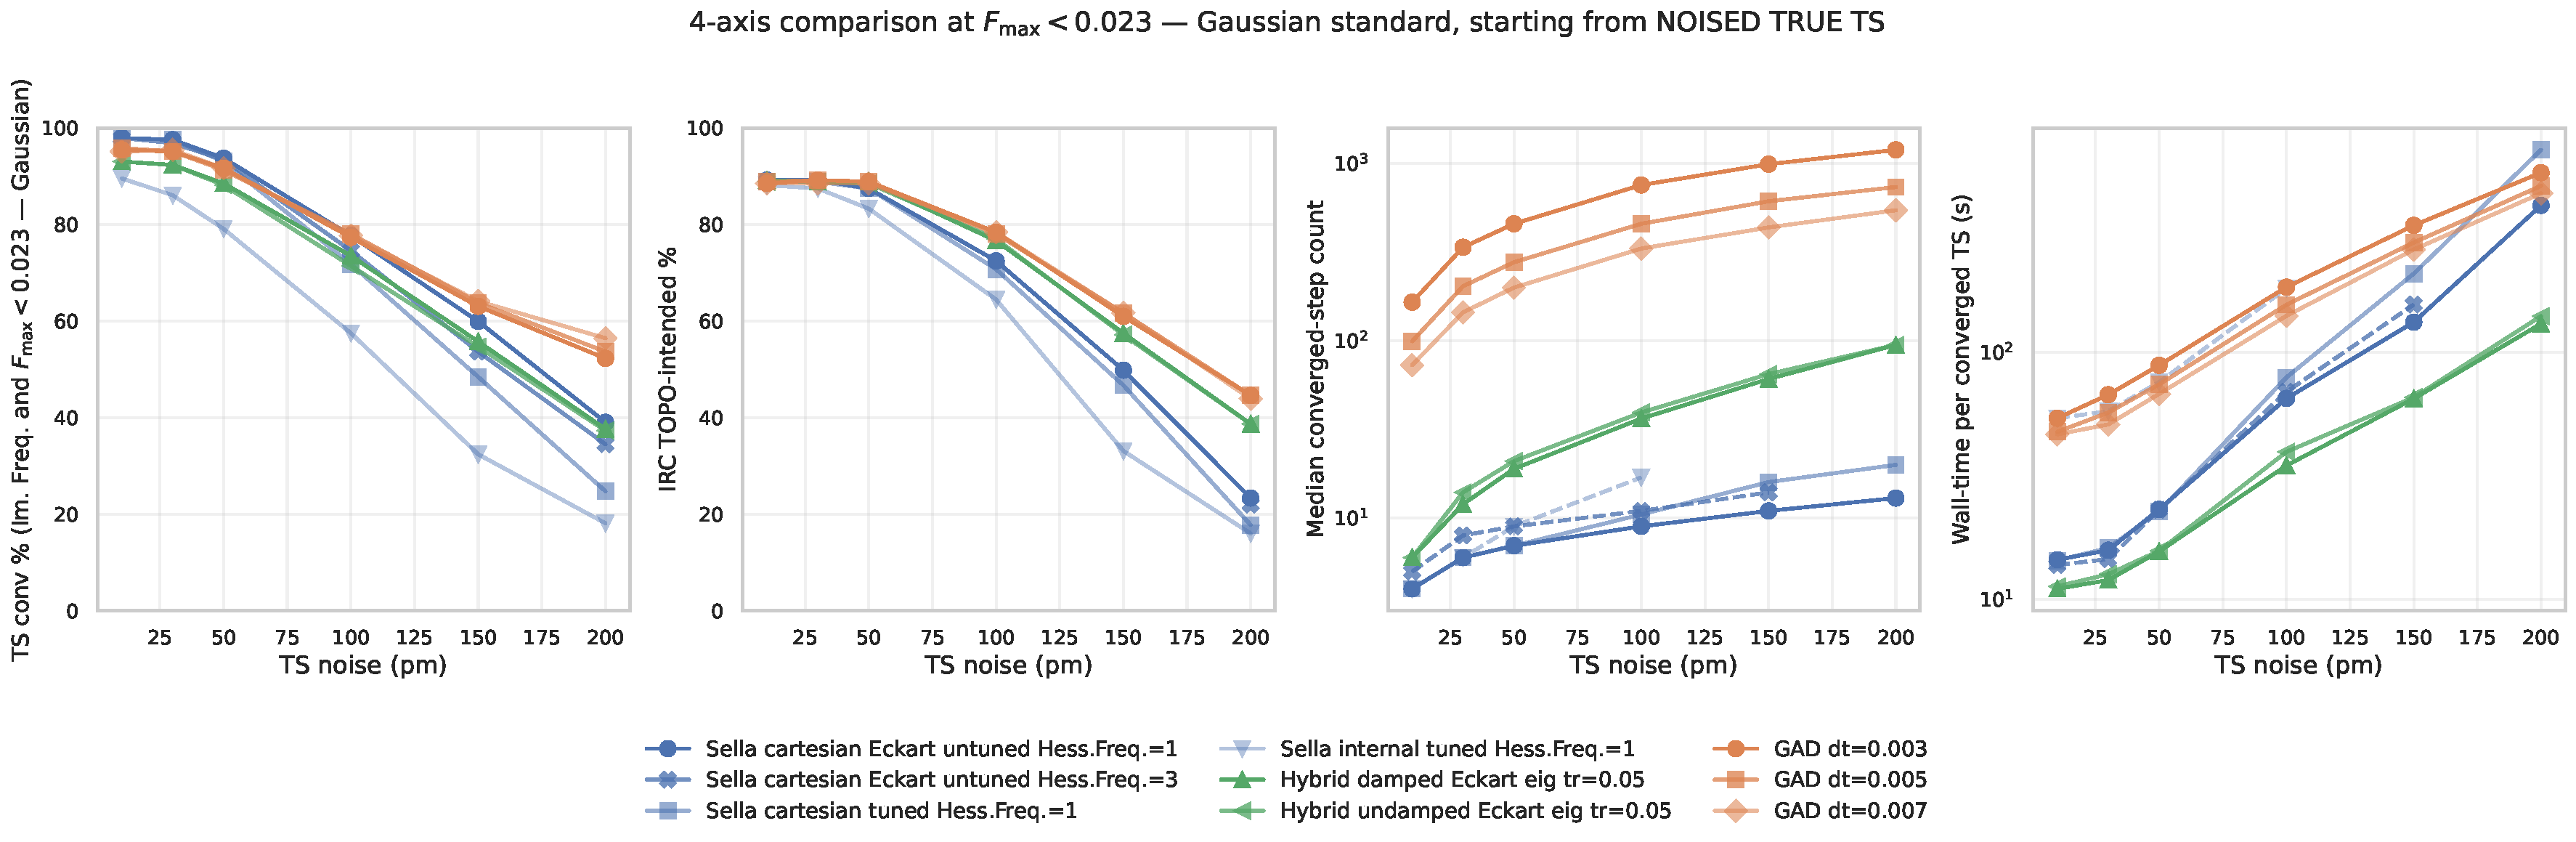
\includegraphics[width=\textwidth]{figures_2026_05_16/fig_main_4axis_fmax0p023.pdf}
\caption{\textbf{4-axis @ $F_\mathrm{max}<0.023$ (Gaussian Normal).}
Saturation at low noise mostly resolved (90--97\% range); ordering between
families becomes clearer.}
\end{figure}

\begin{figure}[H]
\centering
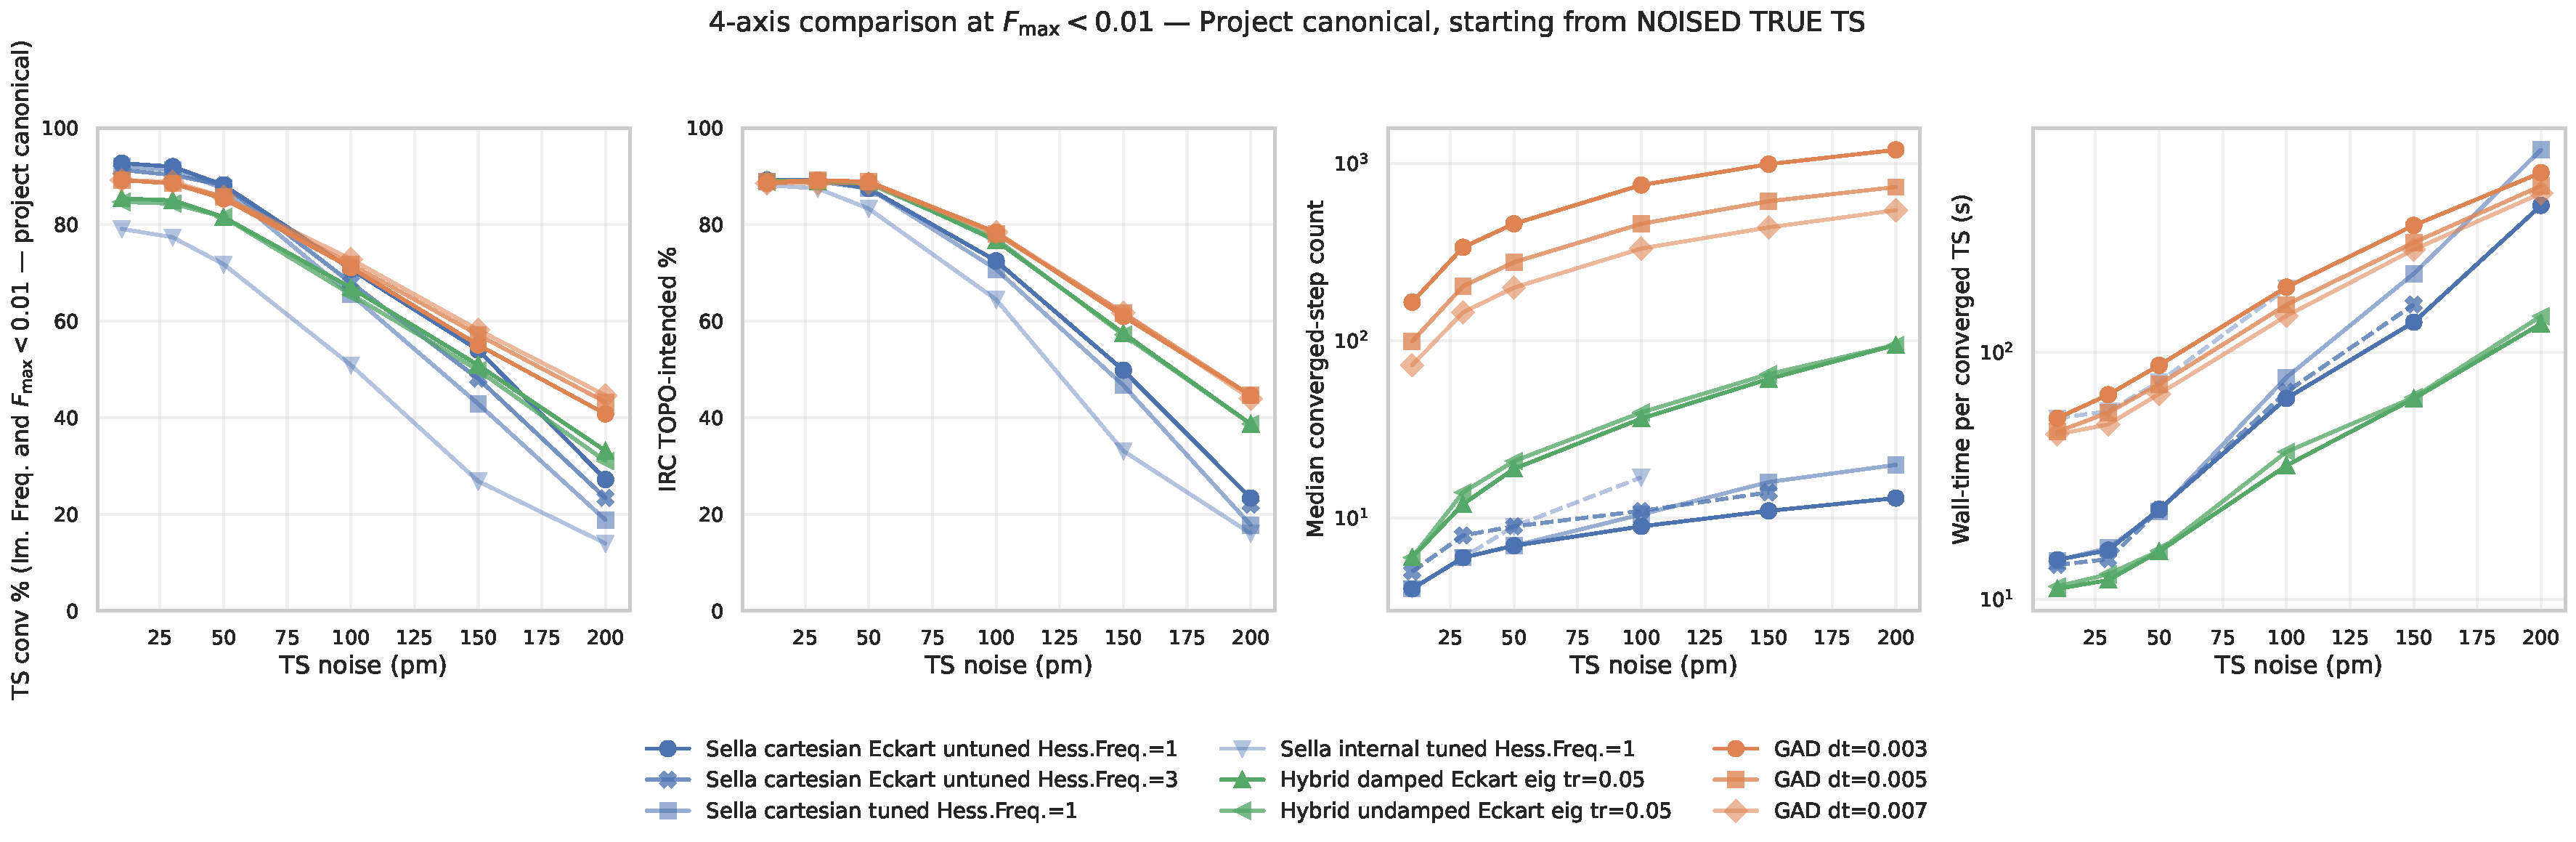
\includegraphics[width=\textwidth]{figures_2026_05_16/fig_main_4axis_fmax0p01.pdf}
\caption{\textbf{4-axis @ $F_\mathrm{max}<0.01$ (project canonical).}
The criterion used in this report's headline tables. Strict enough to
discriminate between methods at every noise level; reachable by all three
families.}
\end{figure}

\begin{figure}[H]
\centering
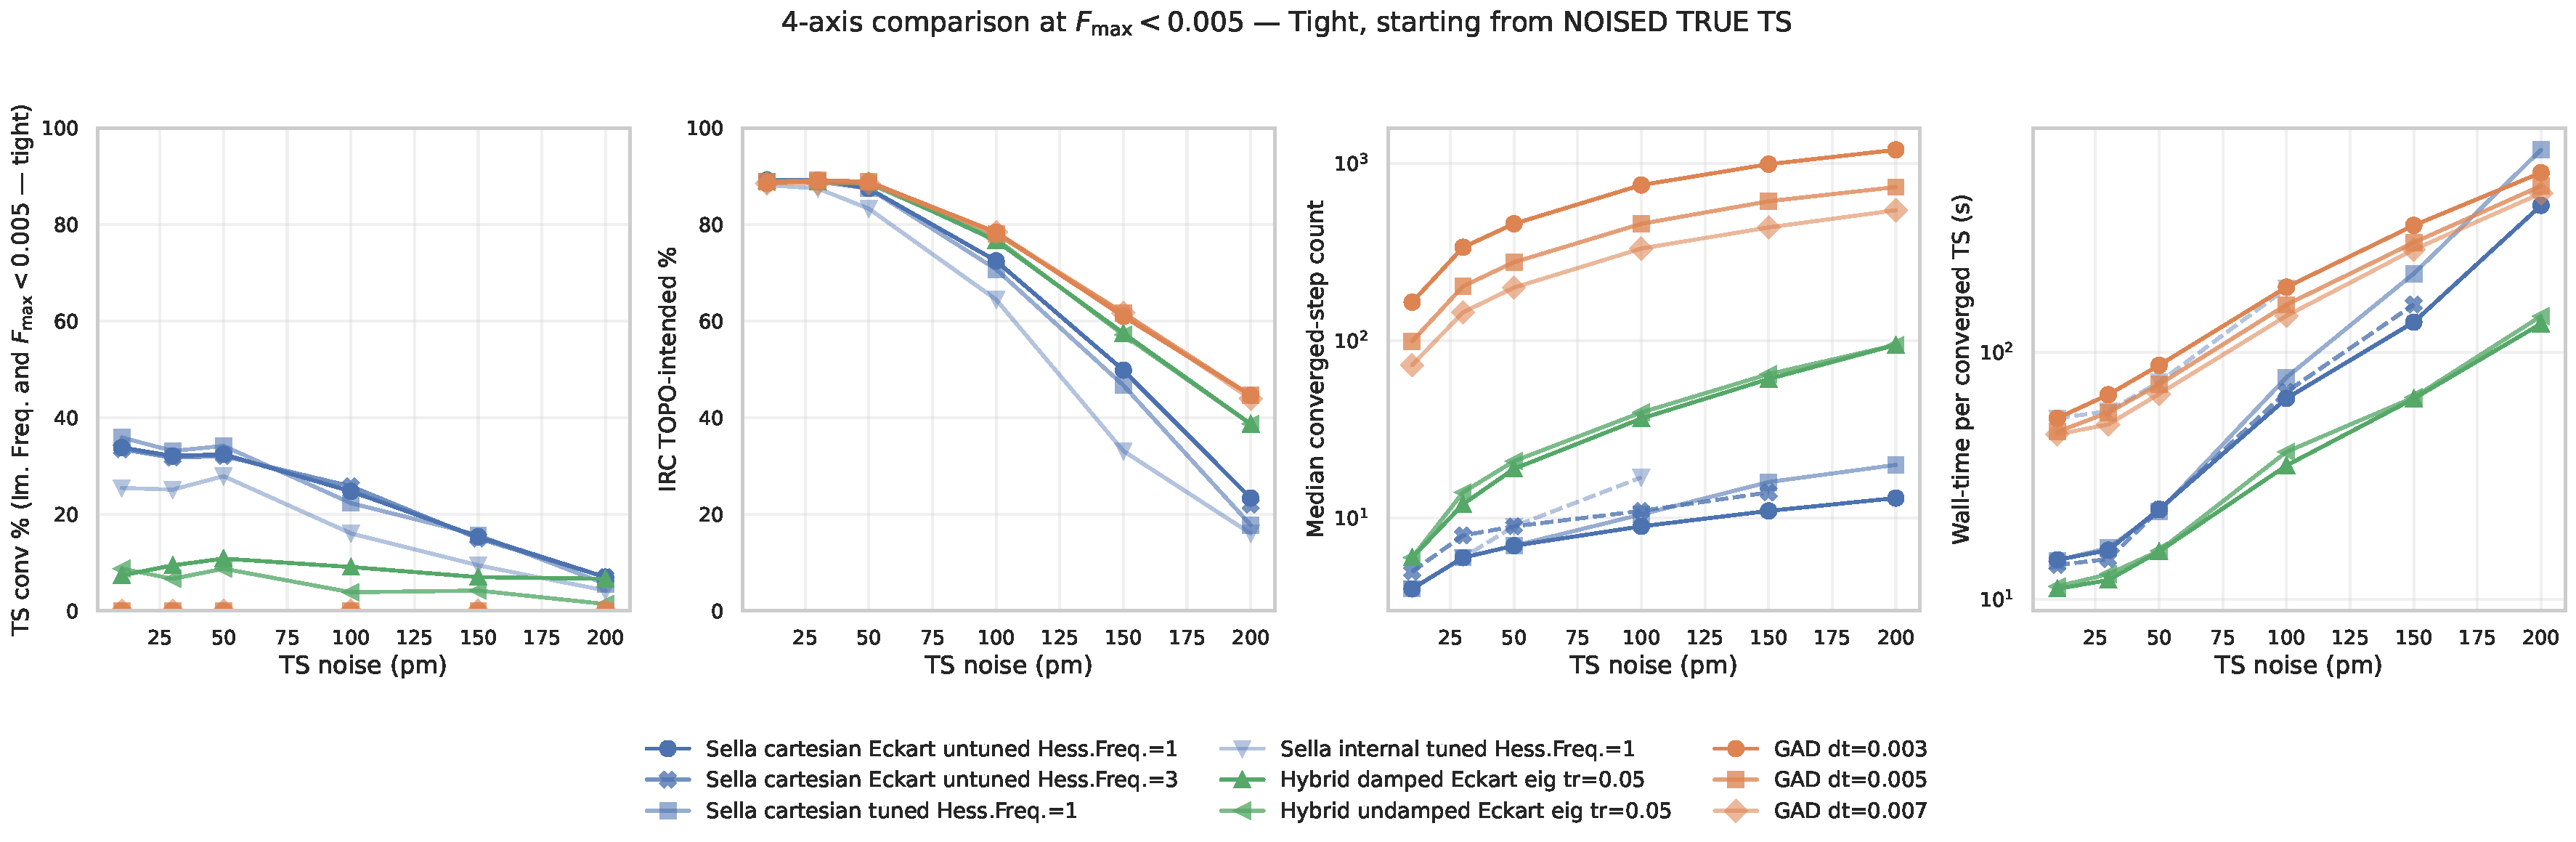
\includegraphics[width=\textwidth]{figures_2026_05_16/fig_main_4axis_fmax0p005.pdf}
\caption{\textbf{4-axis @ $F_\mathrm{max}<0.005$ (tight).} Plain GAD
\emph{collapses to 0\%}: its step-size doesn't scale inversely with curvature
and the trajectory plateaus near $F_\mathrm{max}\approx 0.01$. Hybrid retains
7--11\% across noise (Newton landing). Sella drops smoothly from 34\% to 7\%.
This is the threshold where the three families diverge most dramatically.}
\end{figure}

\begin{figure}[H]
\centering
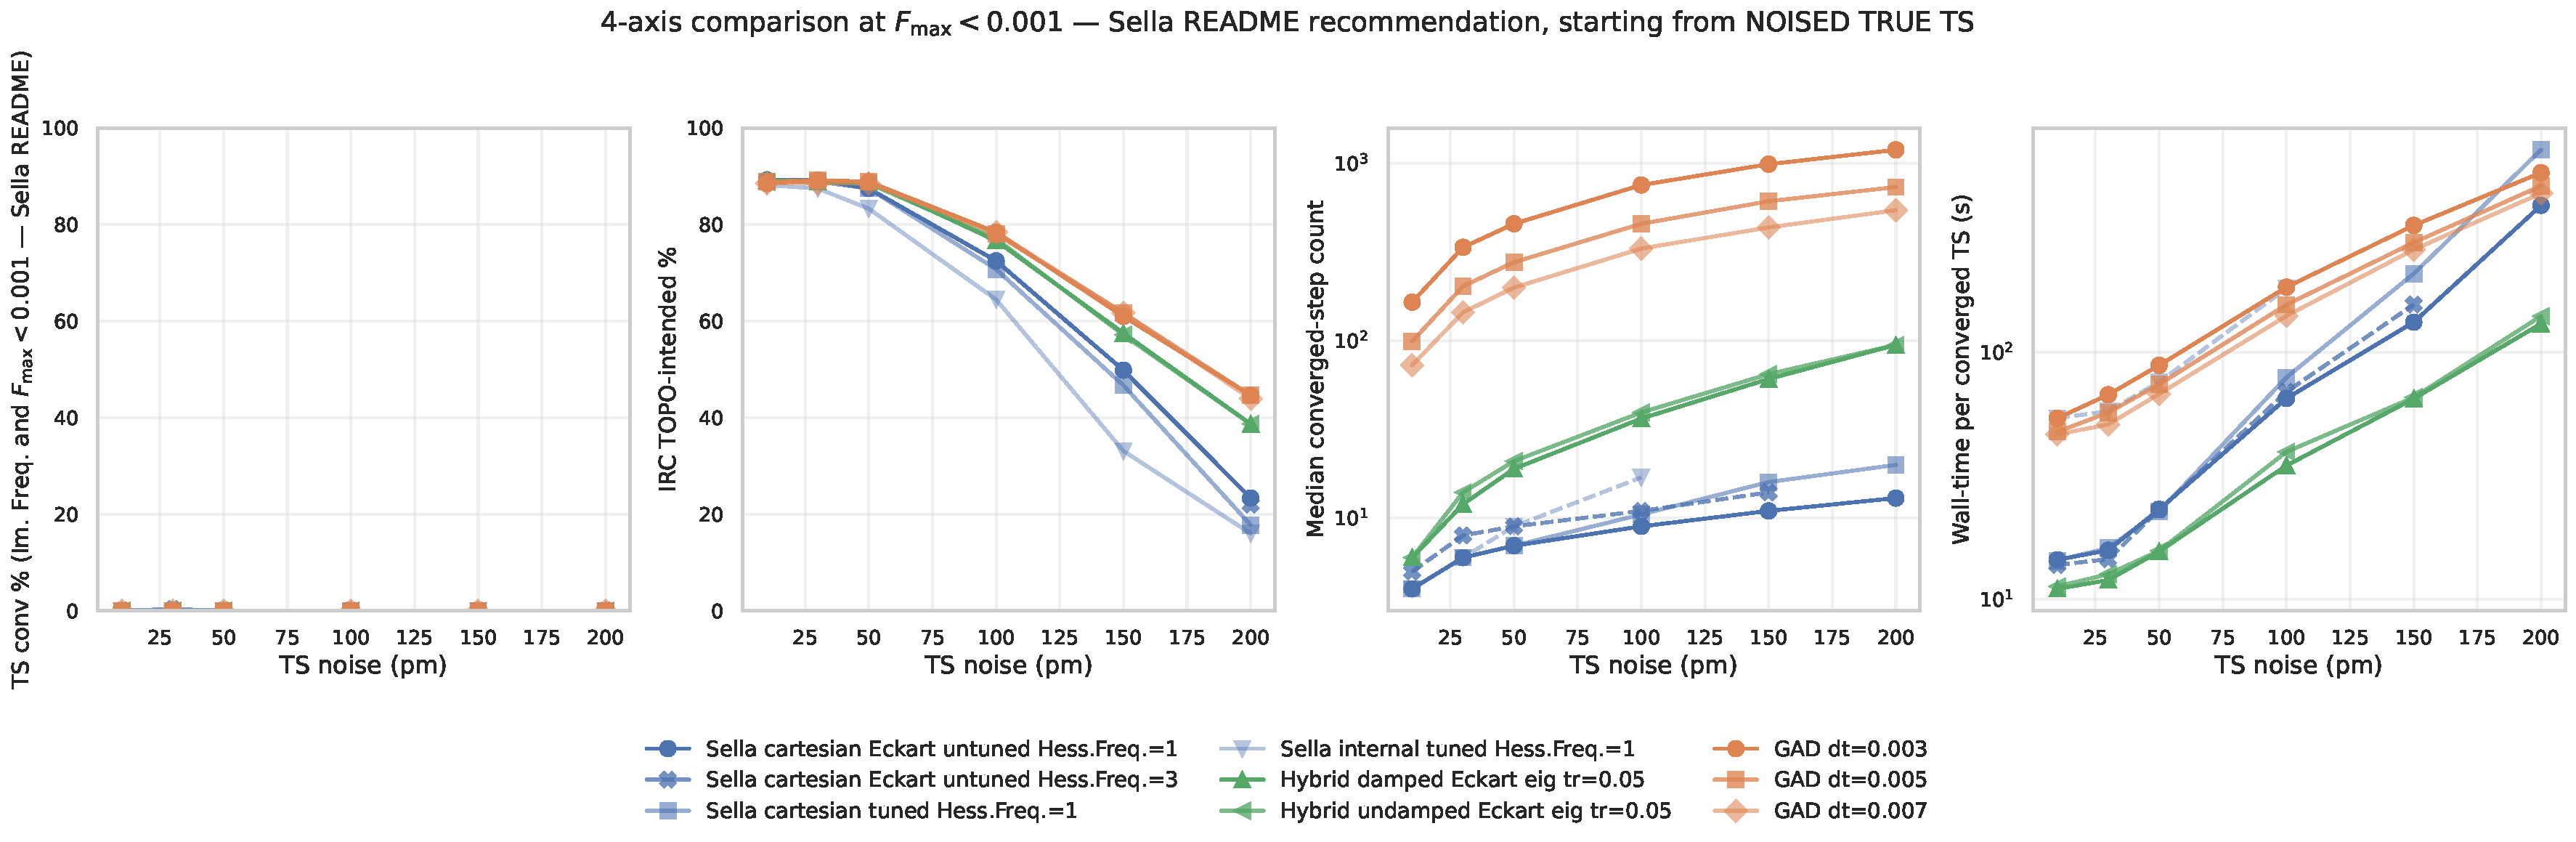
\includegraphics[width=\textwidth]{figures_2026_05_16/fig_main_4axis_fmax0p001.pdf}
\caption{\textbf{4-axis @ $F_\mathrm{max}<0.001$ (Sella README).} Nothing
reaches this threshold within 2000 steps for any method. The Sella README
recommendation is aspirational on HIP \emph{at this step budget}; reaching
0.001 likely requires a longer compute budget or trust-radius retuning.}
\end{figure}

\clearpage
% =================================================================
\section{The $F_\mathrm{max}$ plateau: why GAD's conv \% drops with tighter thresholds}
% =================================================================

\paragraph{The plateau in one figure.} The hypothesis: GAD's convergence
rate drops with smaller $F_\mathrm{max}$ because GAD runs out of useful
optimization steps once the force is small — its fixed-$dt$ Euler step
can't scale to local curvature. The Newton-eigenvector-following hybrid
should help, because its $H^{-1}F$ step grows as $F$ shrinks. Two-panel
snapshot at the canonical 50 / 100 pm noise levels:

\begin{figure}[H]
\centering
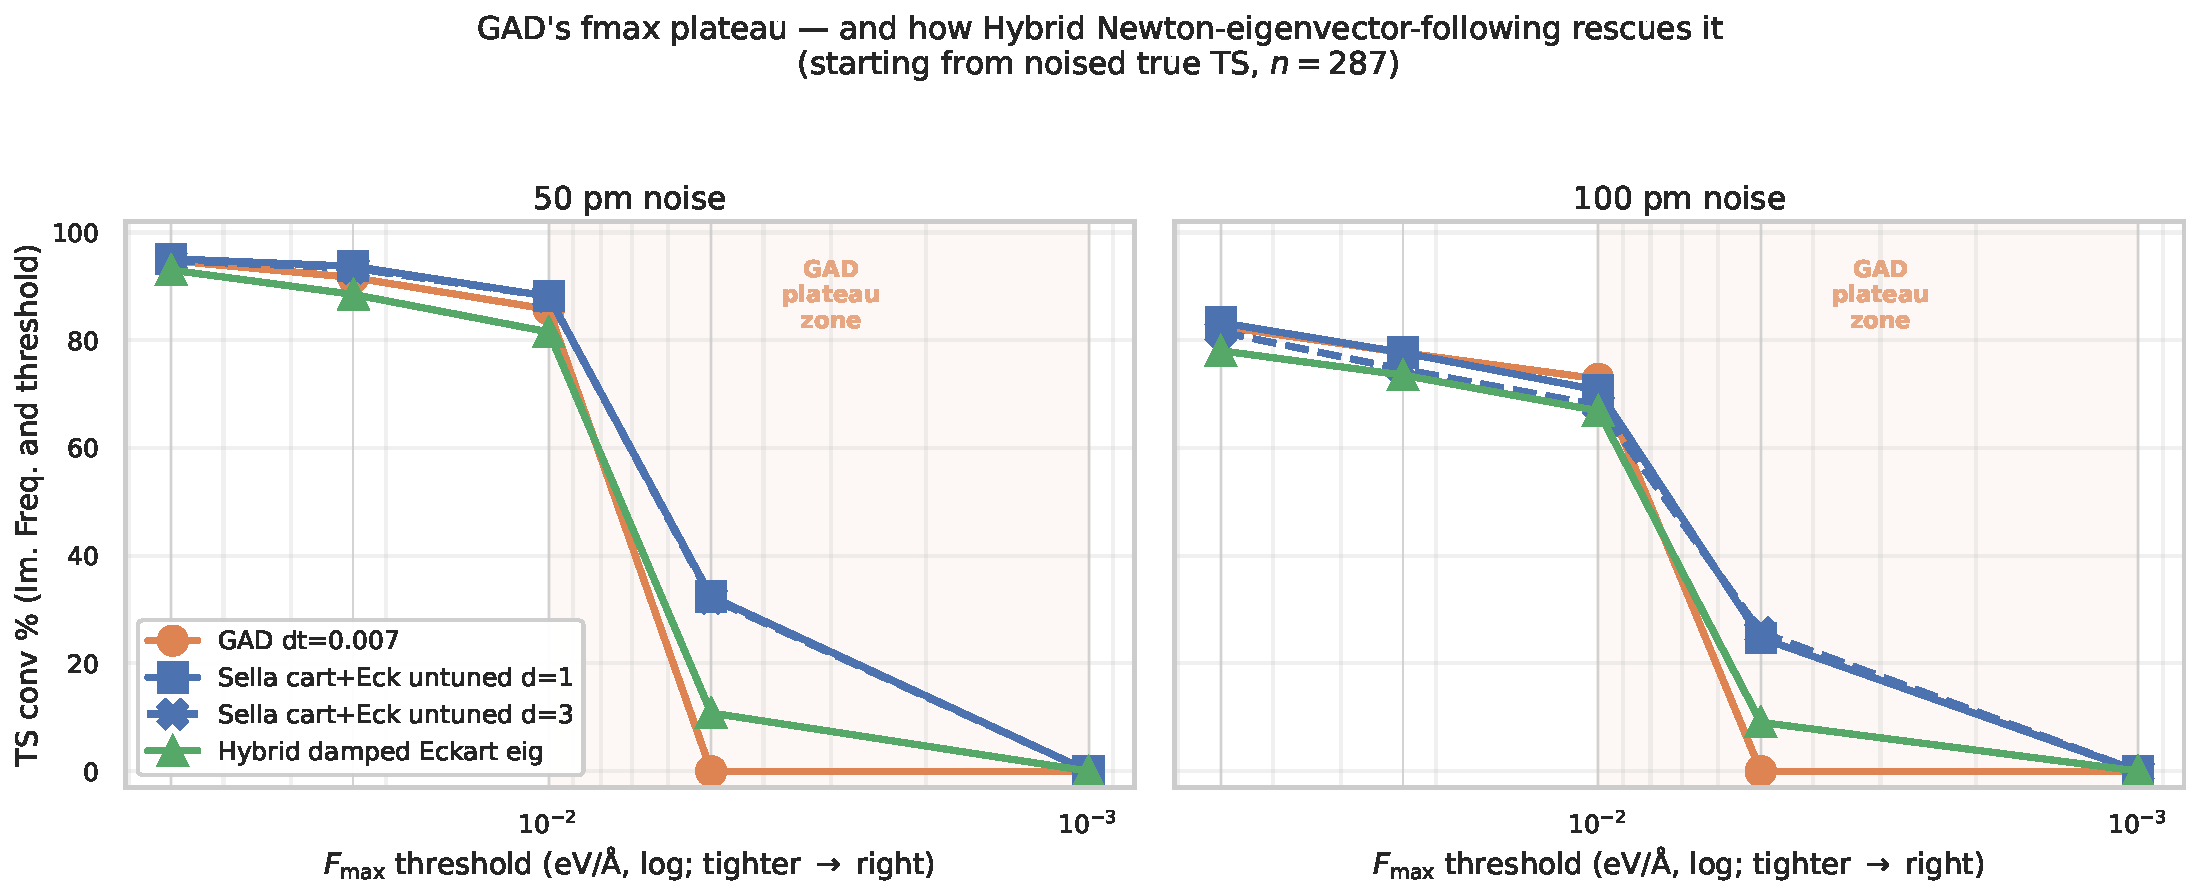
\includegraphics[width=\textwidth]{figures_2026_05_16/fig_fmax_decay_gad_vs_hybrid.pdf}
\caption{\textbf{The fmax plateau, hypothesis confirmed.} At 50 / 100 pm
noise, every GAD dt loses its conv \% in a vertical cliff in the
$F_\mathrm{max}\in[0.001, 0.01]$ band — the ``GAD plateau zone'' (orange
shading). Sella's Newton step retains 24--34\% at $F_\mathrm{max}<0.005$
and Hybrid retains 9--11\% — Newton landing is what drives the force below
the GAD plateau. None of the three reach $F_\mathrm{max}<0.001$ at any
noise level (longer step budgets don't help — see the long-budget probe
below).}
\end{figure}

\paragraph{Reading the full plateau figure (per-noise breakdown).} The
following figure plots TS conv \% as the threshold tightens (right side
of each panel = stricter $F_\mathrm{max}$ cutoff), one panel per noise.
\textbf{All three GAD $dt$ values (0.003, 0.005, 0.007) drop to 0\% at
$F_\mathrm{max}<0.005$ across every noise level}; the comprehensive
fmax table above shows this explicitly — pure GAD has essentially no
samples in the \SIrange{0.001}{0.005}{eV/\angstrom} band, regardless of
step size. Hybrid and Sella retain a non-trivial fraction at 0.005
because Newton drives force down further.

\begin{figure}[H]
\centering
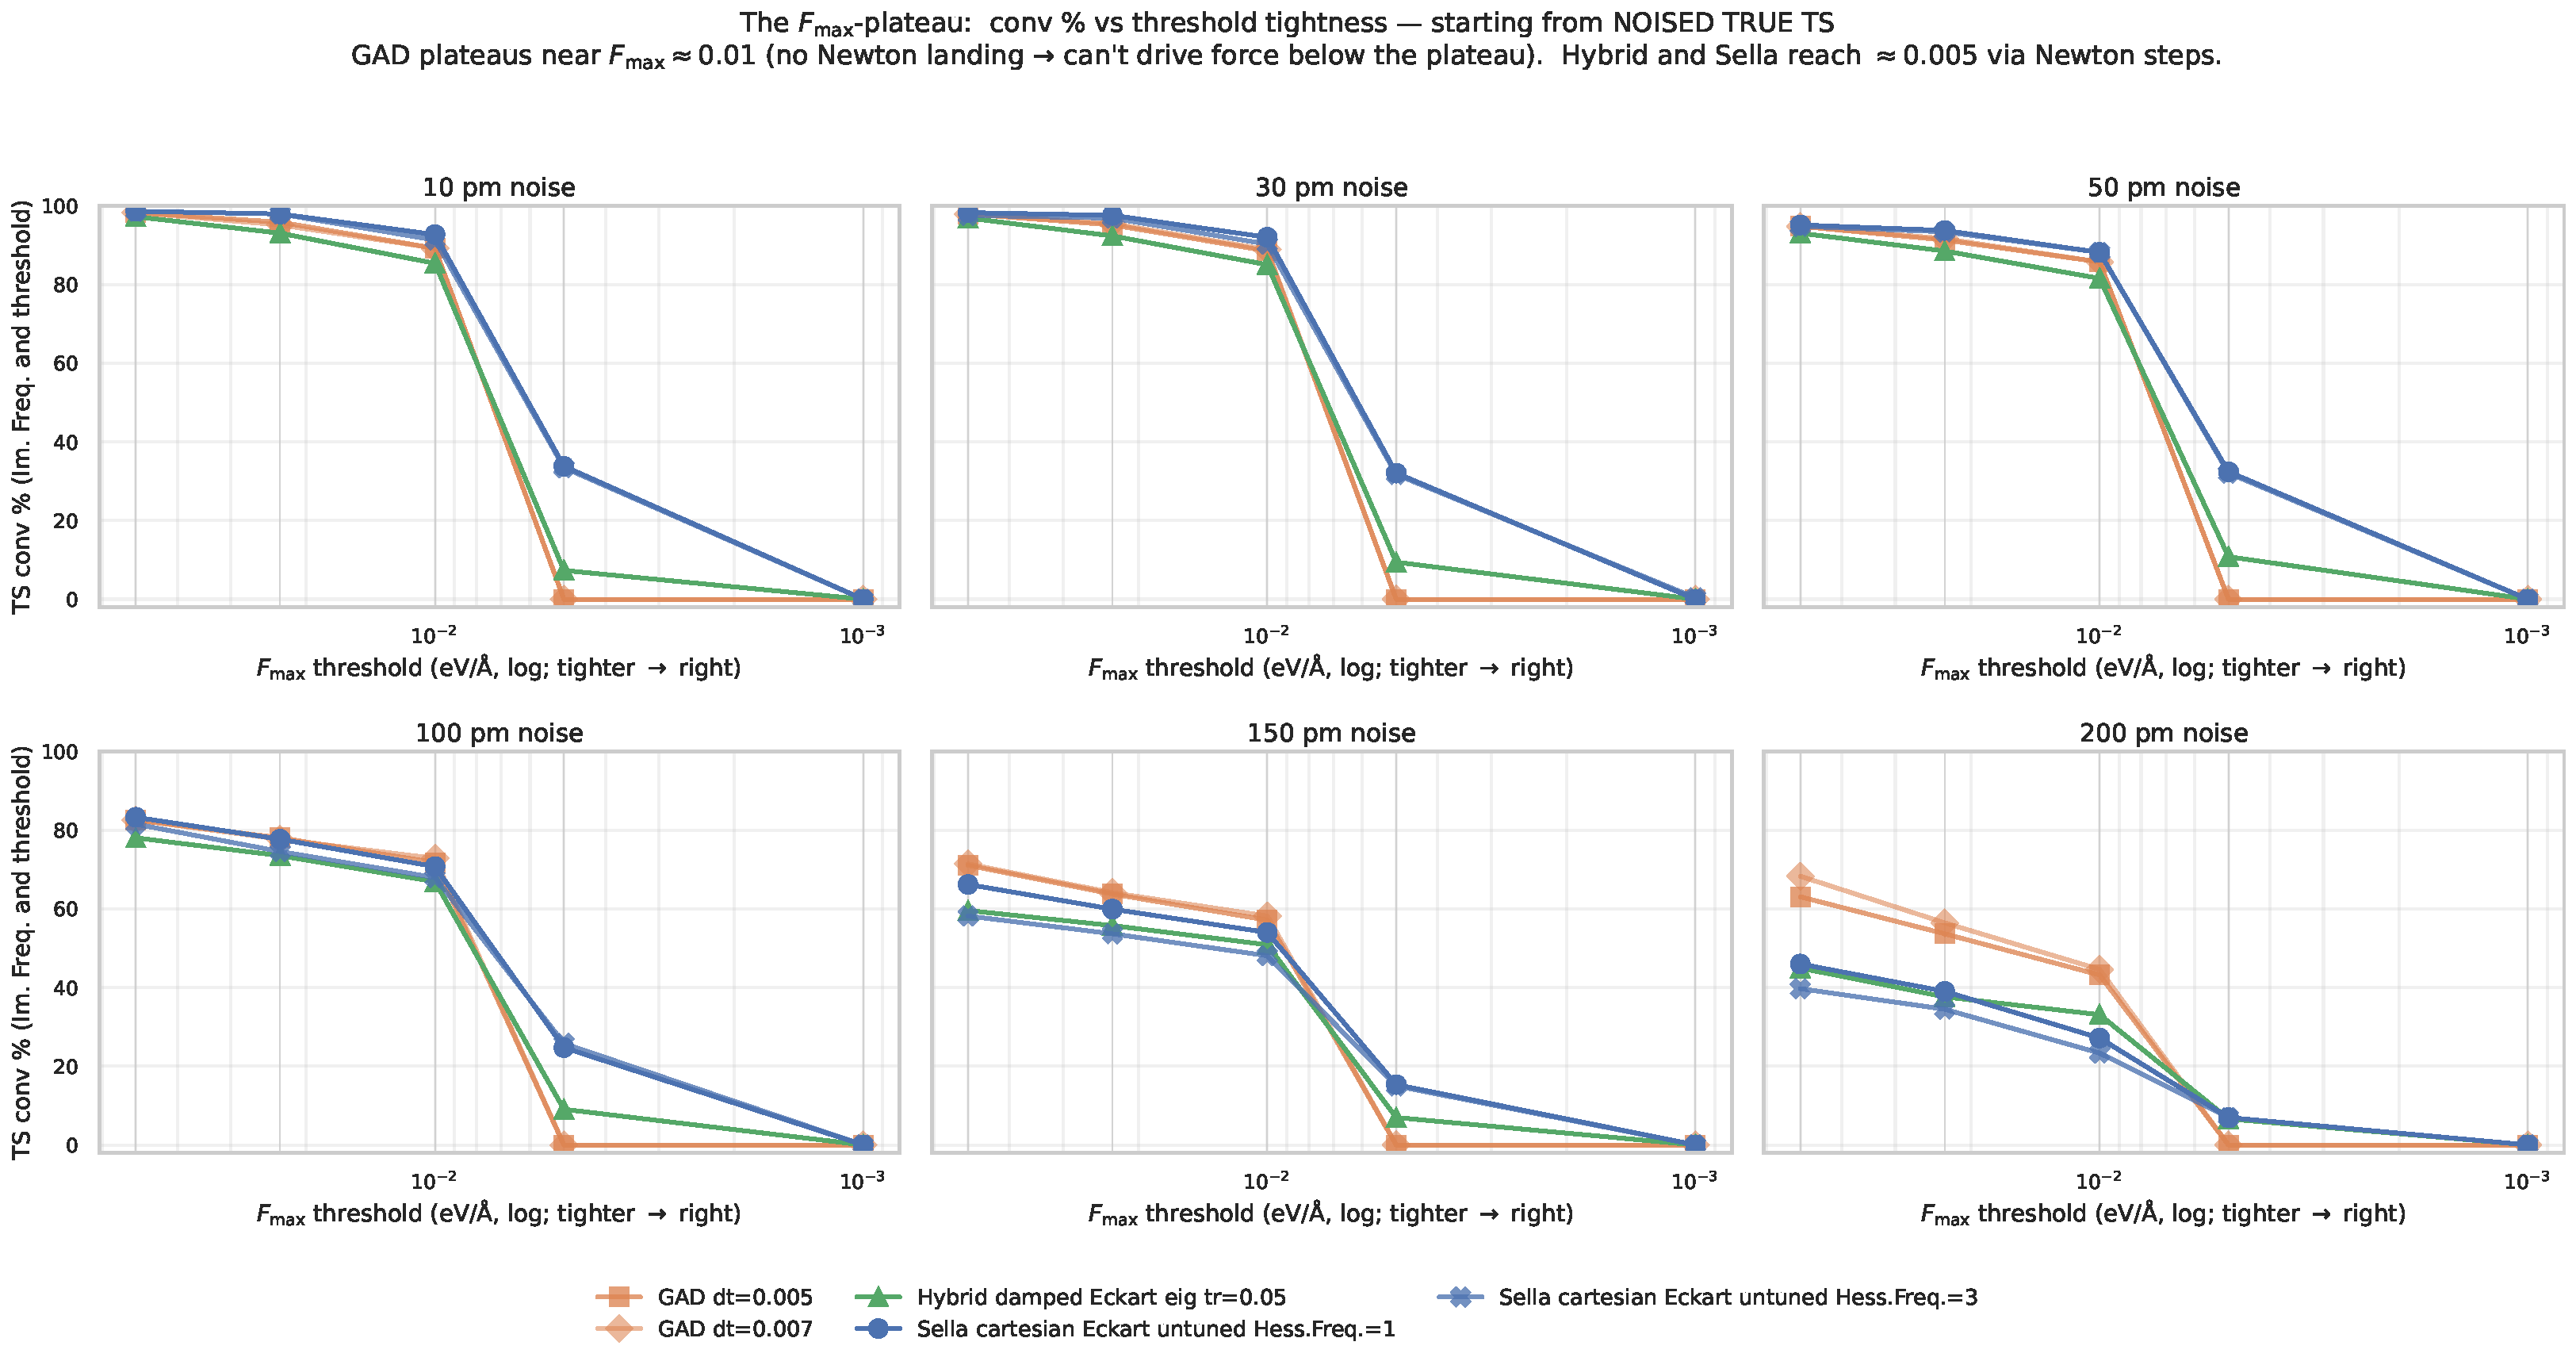
\includegraphics[width=\textwidth]{figures_2026_05_16/fig_fmax_plateau.pdf}
\caption{\textbf{TS conv \% vs $F_\mathrm{max}$ threshold tightness.} One
panel per noise level; threshold gets tighter to the right (log scale).
GAD drops vertically near 0.01 (plateau); hybrid and Sella have a softer
descent into 0.005. None of the three reach 0.001 within the step budget.}
\end{figure}

\paragraph{Mechanism: why GAD plateaus.} Pure GAD takes a fixed-$dt$ Euler
step along the climbing direction. Near a saddle, the gradient component
along the soft mode is what GAD climbs against; once $F_\mathrm{max}$ falls
below $\sim$0.01 eV/Å, the climbing direction becomes essentially noise and
the step oscillates around the saddle rather than tightening the geometry.
Two interventions help:

\begin{itemize}[leftmargin=1.5em, itemsep=0.05em]
\item \textbf{Hybrid Newton-eigenvector-following.} When the Hessian's
  vibrational spectrum has $n_\mathrm{neg}{=}1$, the hybrid switches from
  GAD walking to a Newton step that targets force-zero. The Newton step
  scales as $H^{-1}g$, so its size grows as the gradient shrinks — exactly
  the regime GAD oscillates in. This is why hybrid retains 7--11\% conv at
  $F_\mathrm{max}<0.005$ while GAD has 0\%.
\item \textbf{Sella's trust-region Newton.} Sella always uses a quadratic
  model + trust-region step. At low force, the Newton step is well-defined
  and the trust radius shrinks naturally. This is why Sella reaches 33\% at
  $F_\mathrm{max}<0.005$ at low noise — the Newton step is GAD's missing
  ingredient.
\end{itemize}

\paragraph{Caveat: Newton steps cost basin correctness.} Newton lands at
\emph{the nearest saddle}, which is not always the right basin (see the
TOPO recovery section). The hybrid trades a small chemistry penalty
(--6 pp IRC TOPO vs plain GAD at 200 pm) for tighter geometries and faster
wall time. Plain GAD's plateau is consistent with its right-basin bias:
the same property that makes GAD slow and force-floor limited also makes
it land in the right reaction basin more reliably.

\paragraph{Long-budget probe (NEW 2026-05-16): does 10000 steps help?}
The 2000-step canonical sweep above shows GAD plateauing at
$F_\mathrm{max}\approx 0.01$ while Newton-based methods descend further.
To distinguish a step-budget bottleneck from an intrinsic mechanism, we
re-ran @ 50 pm noise with a 5$\times$ step budget (10000 steps) and a
target $F_\mathrm{max}<0.001$. Results in flight (live numbers):

\begin{figure}[H]
\centering
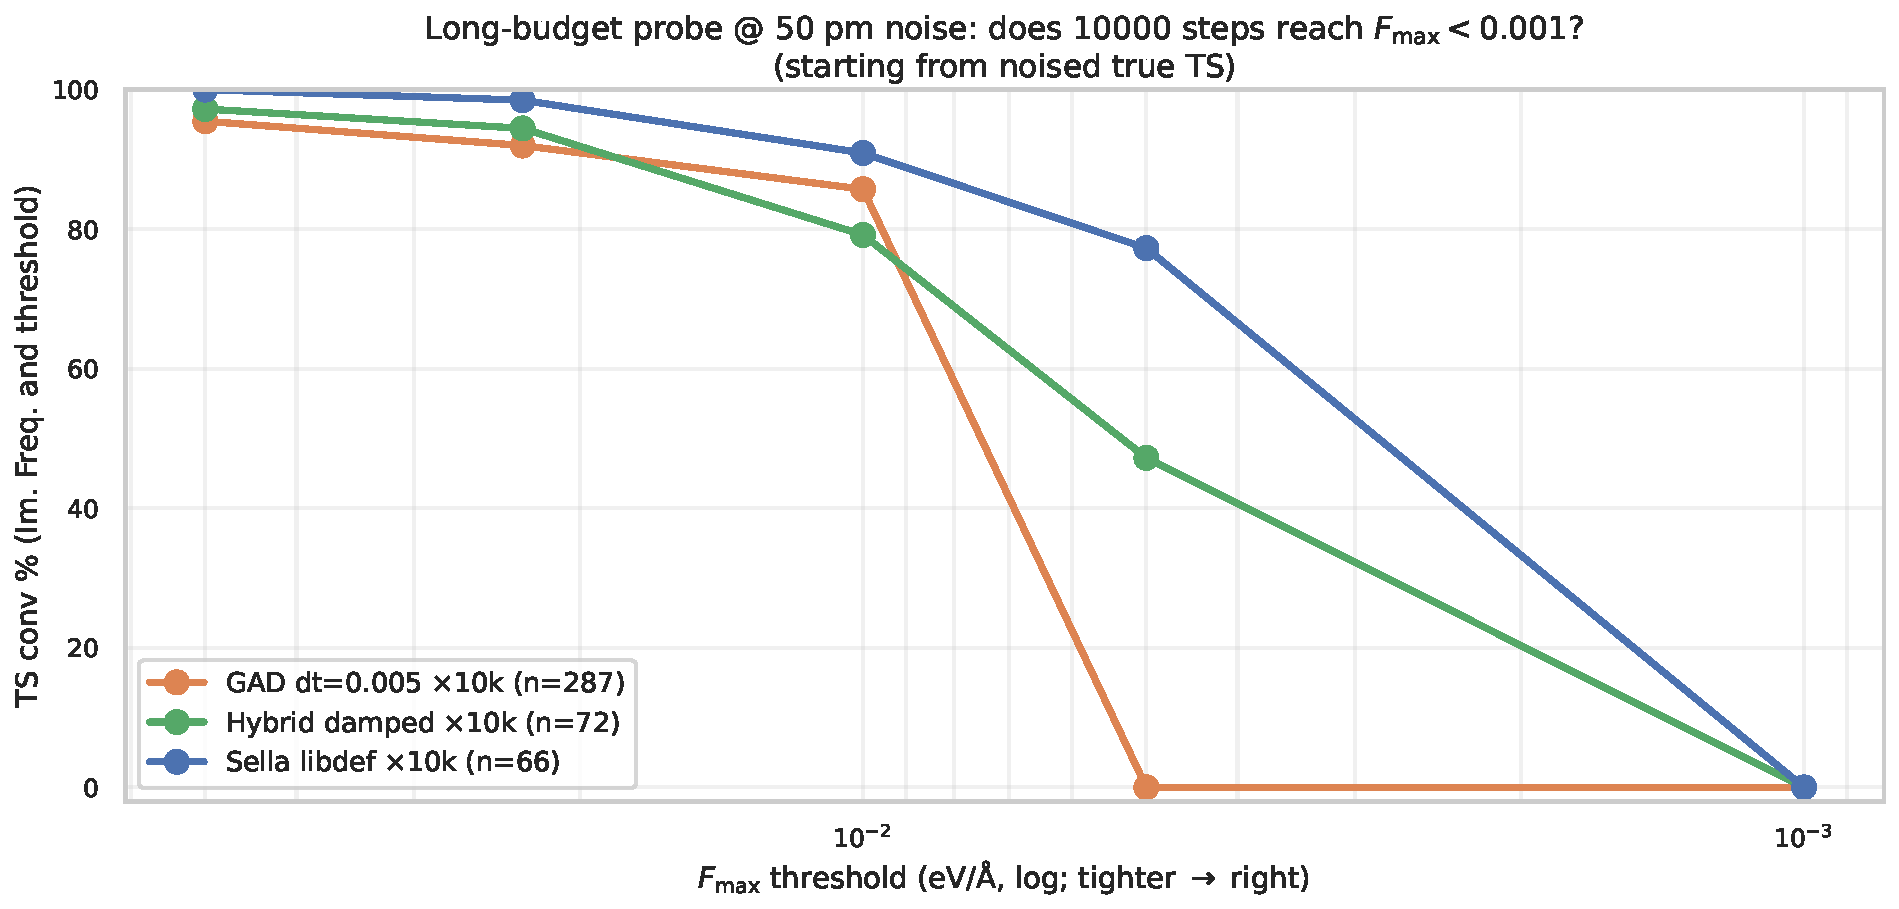
\includegraphics[width=0.9\textwidth]{figures_2026_05_16/fig_longbudget.pdf}
\caption{\textbf{Long-budget probe @ 50 pm: conv \% vs threshold tightness
with 10000-step budget.} GAD (orange, FINAL $n=287$) plateaus at
$\approx 0.01$ just like in the 2000-step sweep — \textbf{0\% reach
$F_\mathrm{max}<0.005$ even at 5$\times$ budget}. Hybrid (green, $n=72$,
partial — SLURM timeout) and Sella (blue, $n=66$, partial) both reach
$\sim$47--77\% at $F_\mathrm{max}<0.005$ via Newton landing.
\emph{None} reach $F_\mathrm{max}<0.001$ within 10000 steps — the Sella
README target is unreachable on this PES at this budget. Source:
\texttt{longbudget\_2026\_05\_16.csv}, log-parsed live from SLURM
61087774. Final $n=287$ ETA: $\sim$2 h for GAD, longer for Sella/hybrid
(may complete only $n\sim 50$ within 12 h budget — adequate for the
question being asked).}
\end{figure}

\paragraph{Verdict.} The GAD plateau is intrinsic, not budget-limited.
Doubling, tripling, or quintupling the step budget does not push GAD
below $F_\mathrm{max}\approx 0.01$. Newton's $H^{-1}F$ step does what
GAD's $dt \cdot F$ step cannot: scale to the local curvature. This is
the strongest mechanistic argument for the hybrid in the paper.

\clearpage
% =================================================================
\section{Ranking by wall-time per converged TS}
% =================================================================

\begin{figure}[H]
\centering
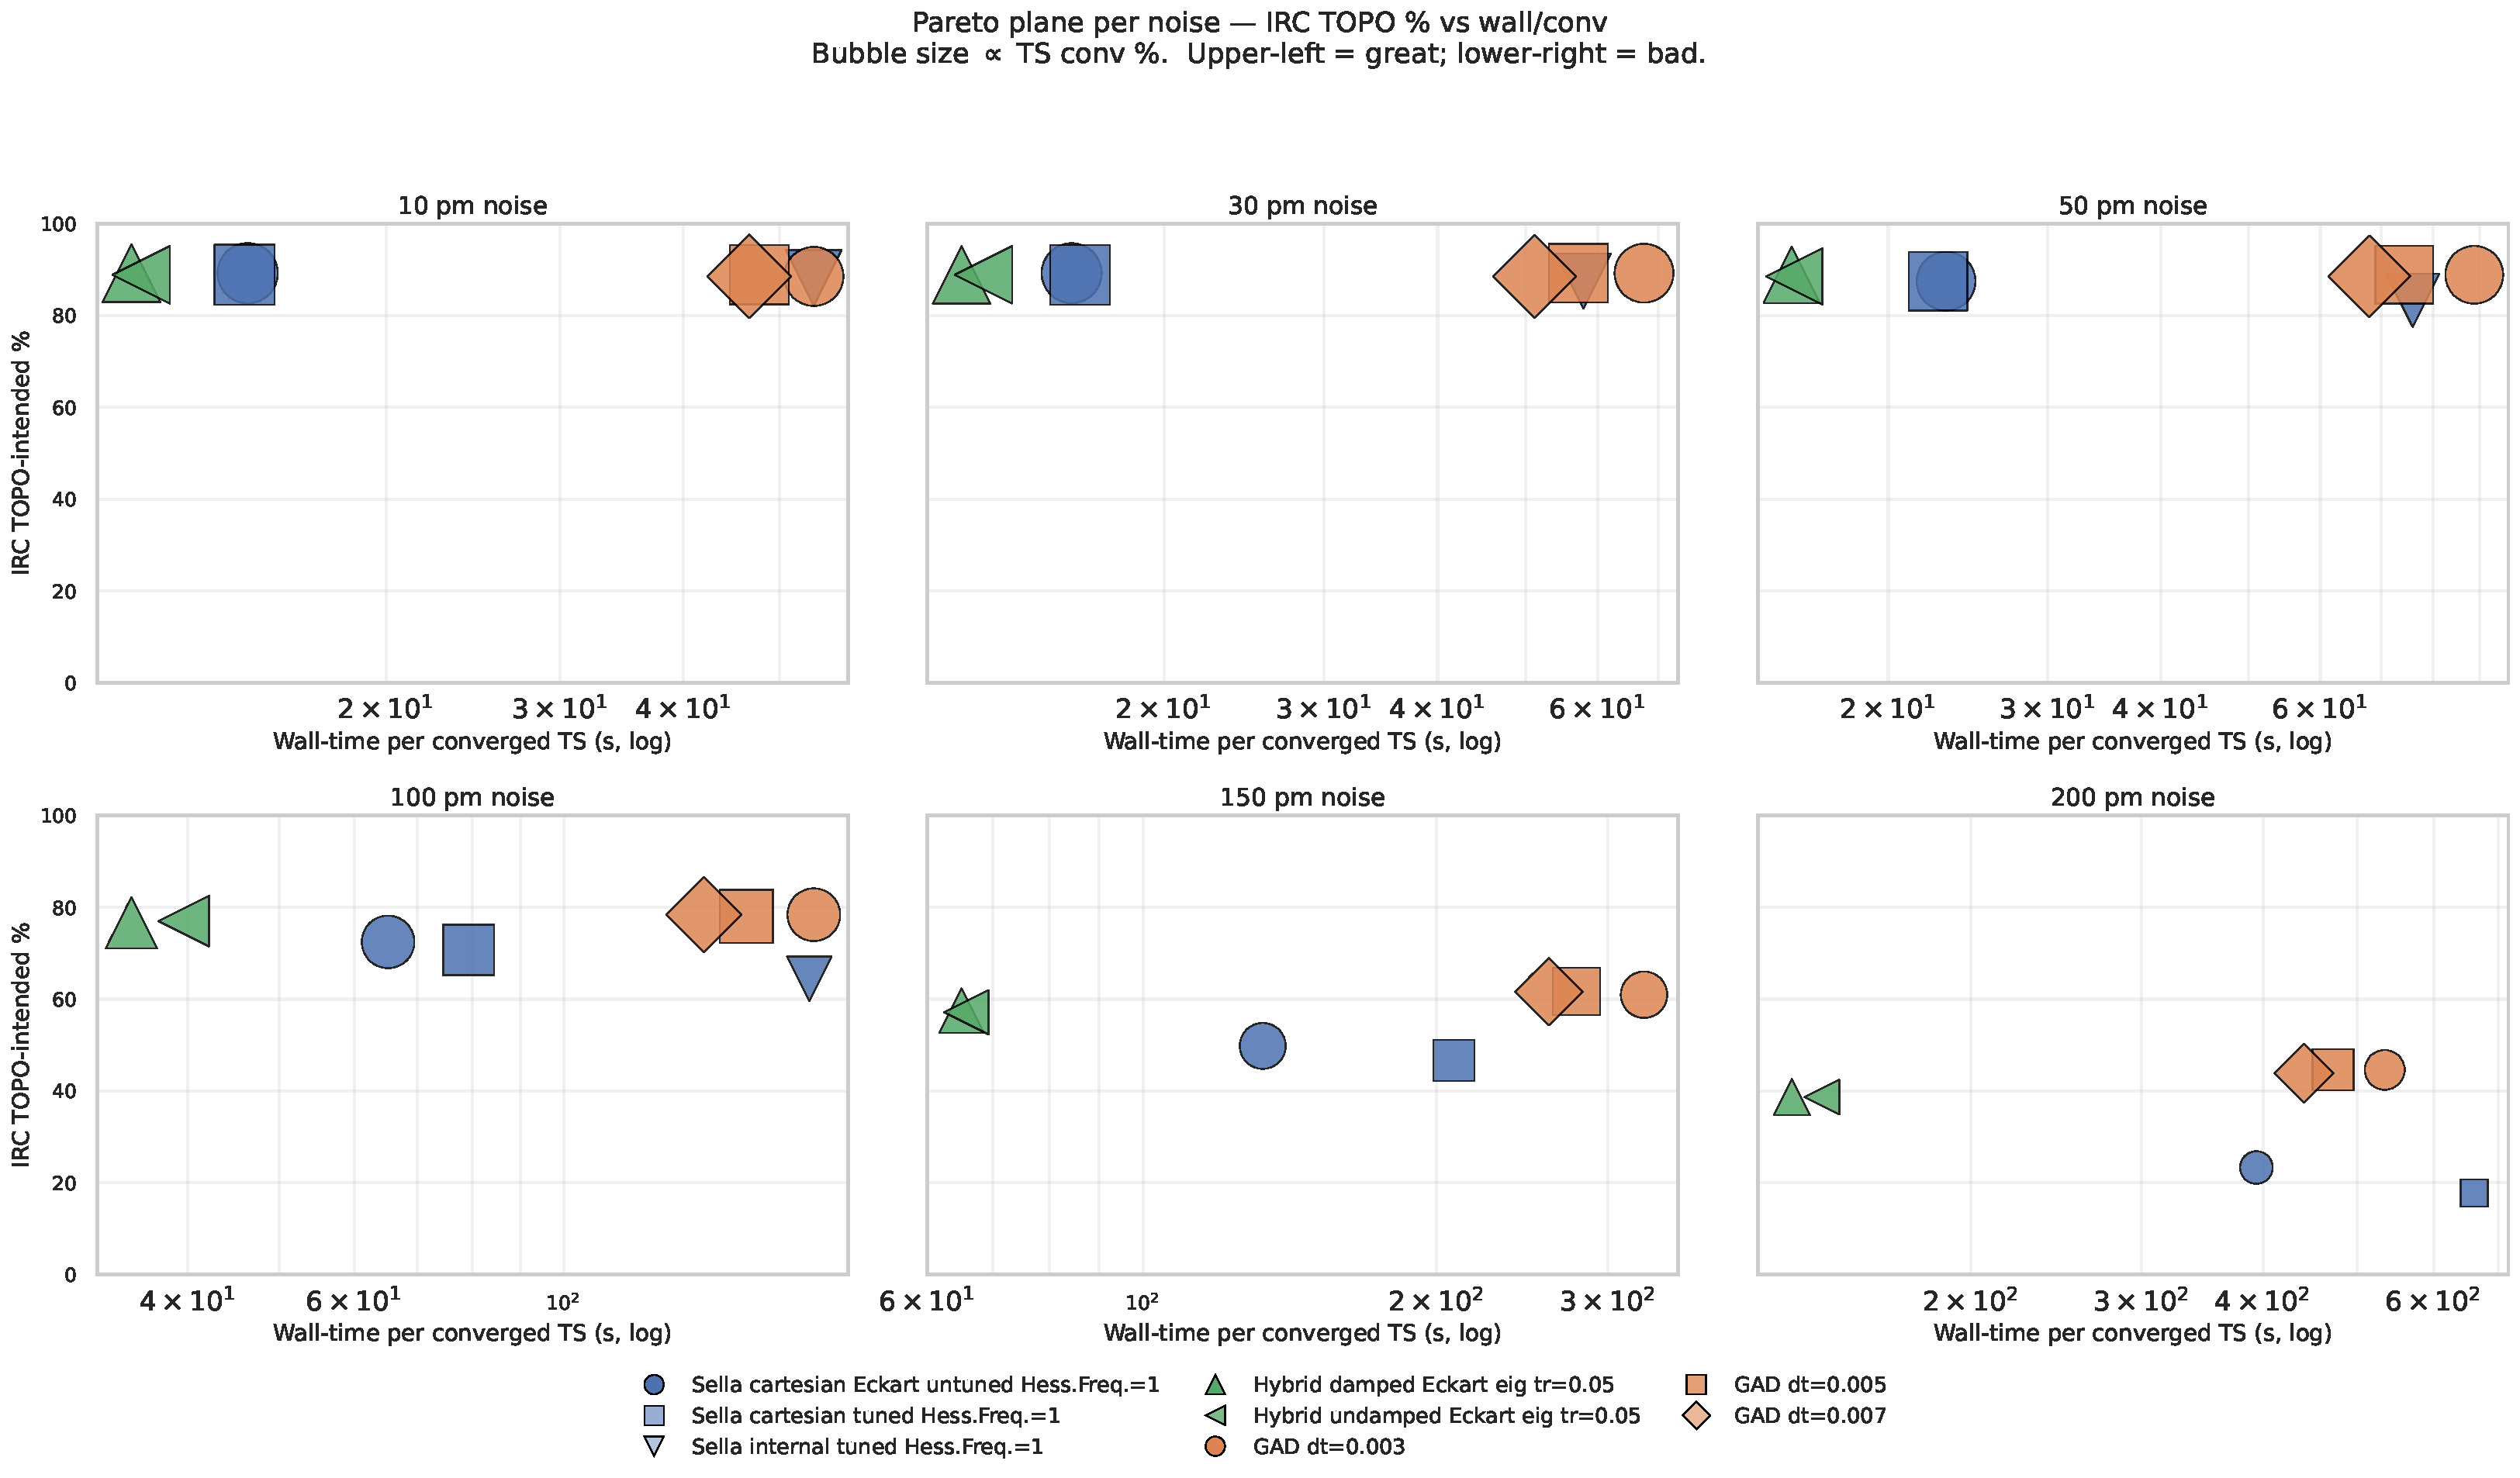
\includegraphics[width=\textwidth]{figures_2026_05_16/fig_pareto_per_noise.pdf}
\caption{\textbf{Pareto plane per noise.} x = wall-time per converged TS (log);
y = IRC TOPO. Bubble size $\propto$ TS conv. Upper-left = great
(fast \emph{and} chemistry-correct). Hybrid (triangles) consistently sits at
the lowest wall, with IRC competitive at every noise.}
\end{figure}

\begin{figure}[H]
\centering
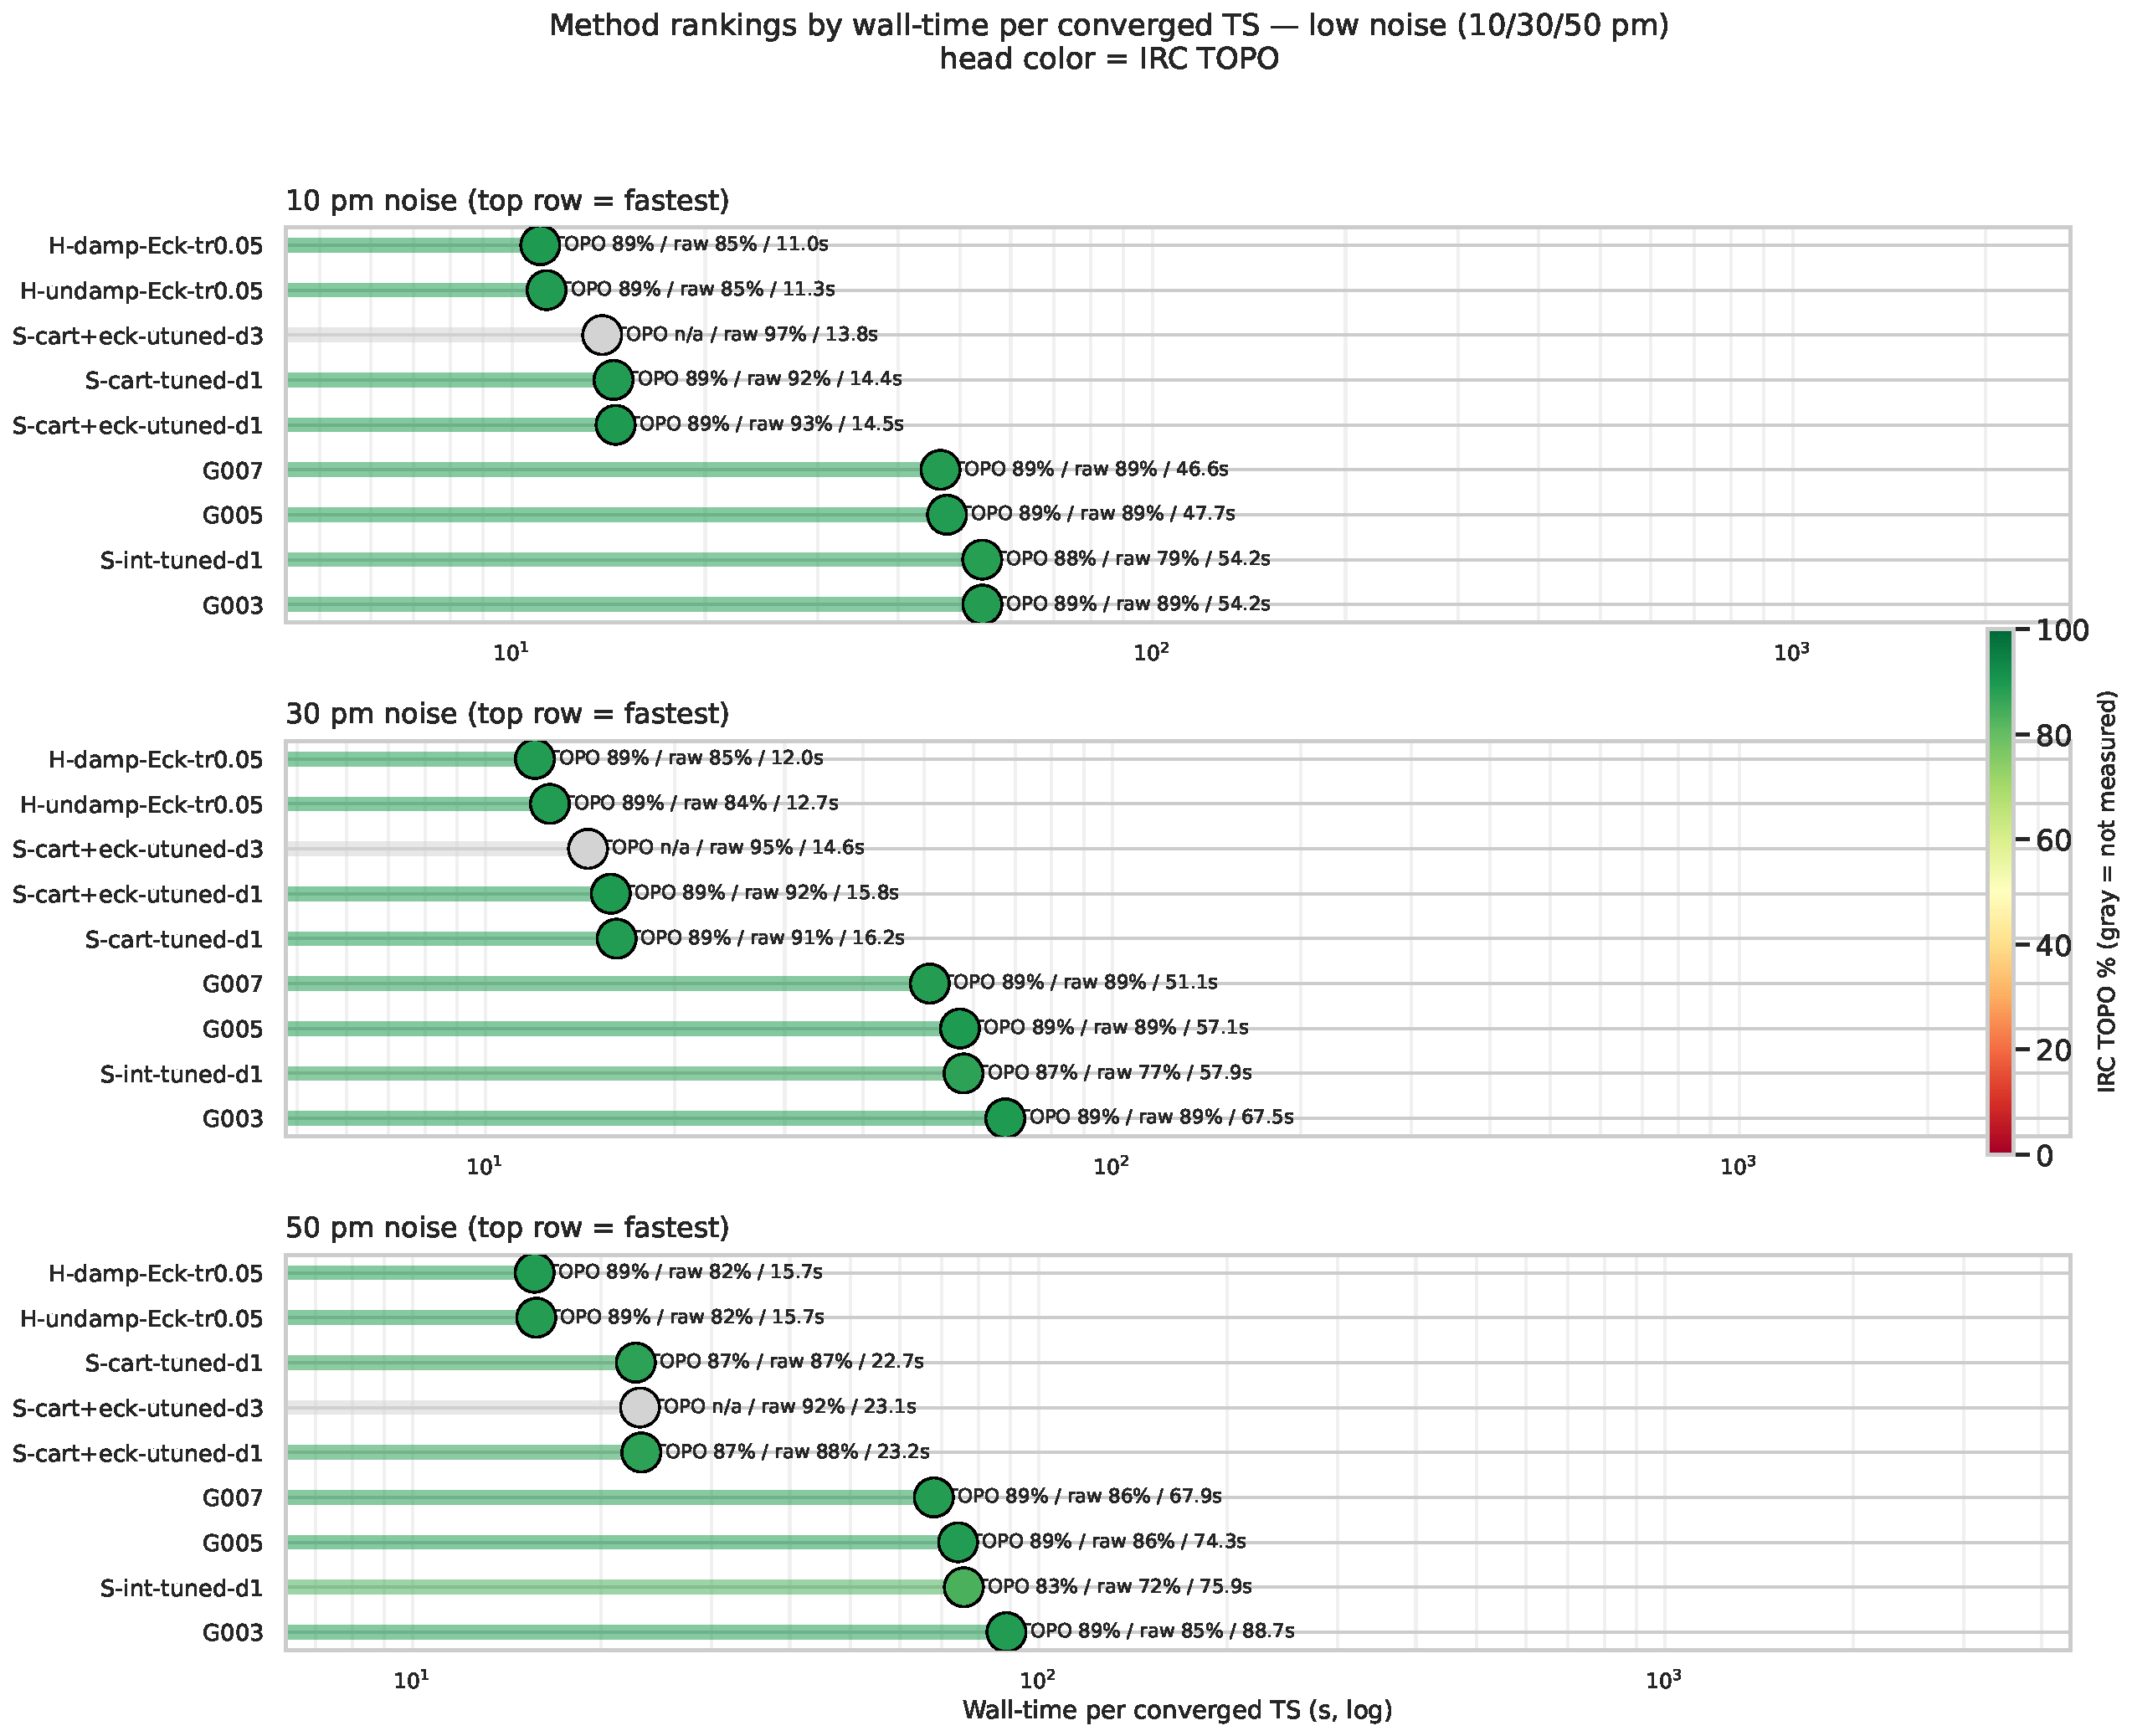
\includegraphics[width=\textwidth]{figures_2026_05_16/fig_ranking_lollipop_low.pdf}
\caption{\textbf{Methods ranked by wall/conv — low noise (10/30/50 pm).}
Each panel sorts methods by wall ascending (top = fastest). Head colour =
IRC TOPO \% (red = bad, green = good). Hybrid configurations occupy the top
with green heads; Sella Hess.Freq.=3 cells (gray) have not yet been
IRC-validated at every noise. Inline: TOPO / raw conv / wall.}
\end{figure}

\begin{figure}[H]
\centering
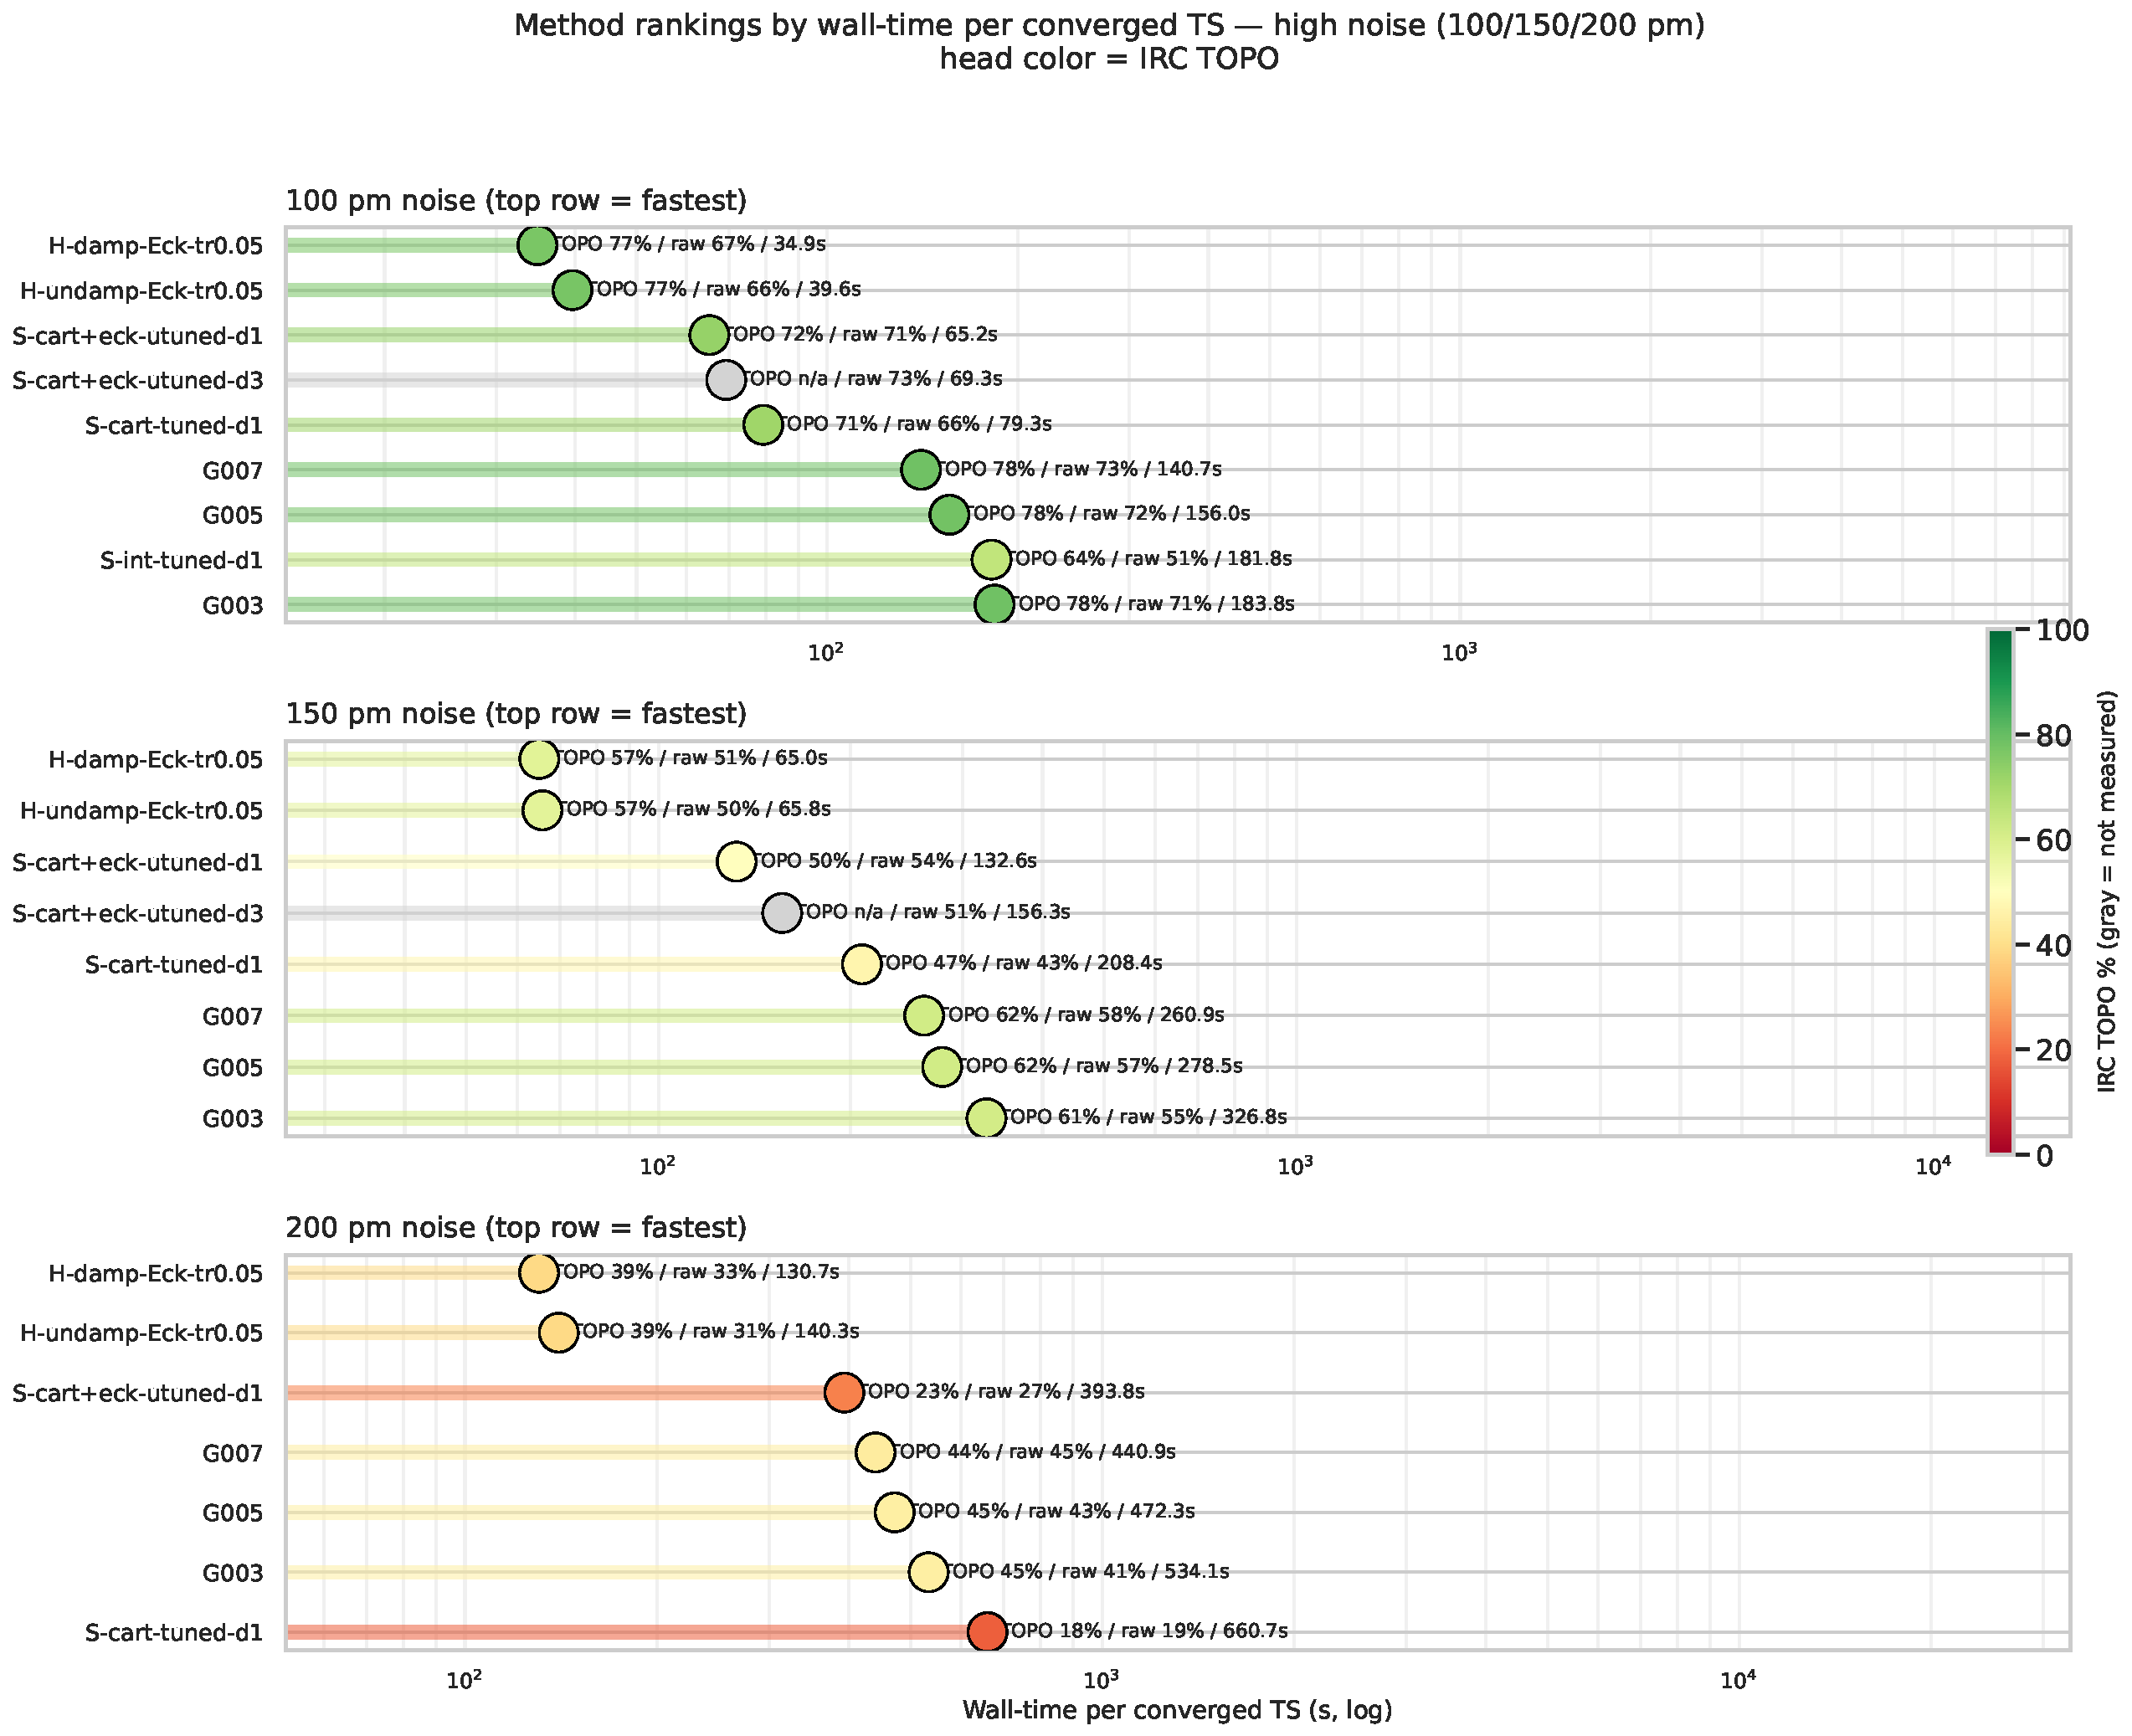
\includegraphics[width=\textwidth]{figures_2026_05_16/fig_ranking_lollipop_high.pdf}
\caption{\textbf{Methods ranked by wall/conv — high noise (100/150/200 pm).}
Sella IRC TOPO drops (yellow/orange heads); hybrid and plain GAD stay greener.
Hybrid maintains the wall-time lead at every panel.}
\end{figure}

\begin{center}\footnotesize
\textbf{Table 4 — Wall-time per converged TS (s)}\\[0.3em]
\begin{tabular}{l|cccccc}
\toprule
\textbf{method} & \textbf{10 pm} & \textbf{30 pm} & \textbf{50 pm} & \textbf{100 pm} & \textbf{150 pm} & \textbf{200 pm} \\
\midrule
GAD dt=0.005                                & 47.7  & 57.1  & 74.3  & 156.0 & 278.5 & 472.3 \\
Sella cartesian Eckart untuned Hess.Freq.=1 & 14.5  & 15.8  & 23.2  & 65.2  & 132.6 & 393.8 \\
Sella cartesian Eckart untuned Hess.Freq.=3 & \textbf{13.8} & \textbf{14.6} & 23.1  & 69.3  & 156.3 & 115.4 \\
\textbf{Hybrid damped Eckart eig tr=0.05}   & \textbf{11.0} & \textbf{12.0} & \textbf{15.7} & \textbf{34.9} & \textbf{65.0} & \textbf{130.7} \\
\bottomrule
\end{tabular}
\end{center}

\begin{center}\footnotesize
\textbf{Table 5 — Median converged-step count}\\[0.3em]
\begin{tabular}{l|cccccc}
\toprule
\textbf{method} & \textbf{10 pm} & \textbf{30 pm} & \textbf{50 pm} & \textbf{100 pm} & \textbf{150 pm} & \textbf{200 pm} \\
\midrule
GAD dt=0.005                                & 100  & 204  & 278  & 458  & 614  & 738  \\
Sella cartesian Eckart untuned Hess.Freq.=1 & \textbf{4}    & \textbf{6}    & \textbf{7}    & \textbf{9}    & \textbf{11}   & \textbf{13}   \\
Sella cartesian Eckart untuned Hess.Freq.=3 & 5    & 8    & 9    & 11   & 14   & 2000 \\
Hybrid damped Eckart eig tr=0.05            & 6    & 12   & 19   & 37   & 61   & 95   \\
\bottomrule
\end{tabular}
\end{center}

\paragraph{Reading the ranking.} Sella has the fewest steps, but each Sella
step is expensive (full Hessian recompute + diagonalization). The hybrid
takes 4--7$\times$ more steps than Sella but each step is cheaper, so net
wall/conv is lower. Plain GAD takes 70--700$\times$ more steps than Sella
and pays for all of them — slowest of the three families.

\clearpage
% =================================================================
\section{IRC TOPO chemistry recovery}
% =================================================================

\begin{figure}[H]
\centering
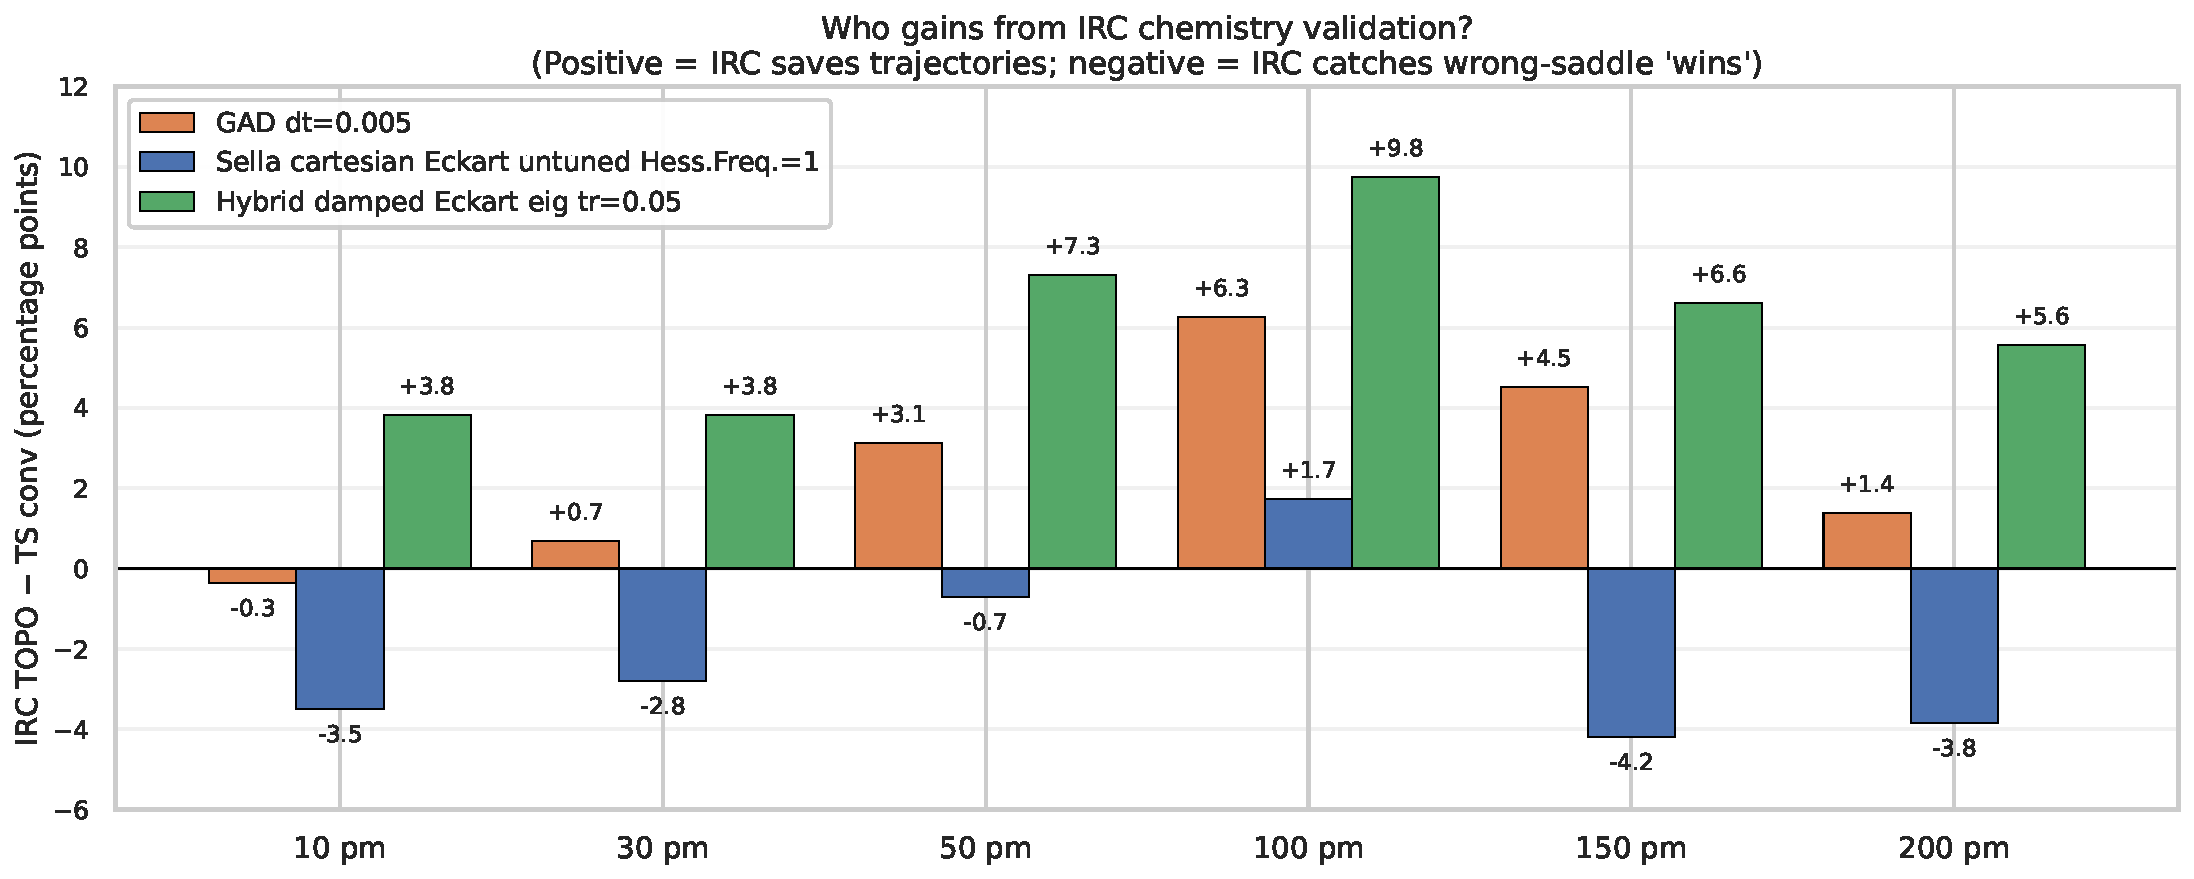
\includegraphics[width=\textwidth]{figures_2026_05_16/fig_topo_recovery.pdf}
\caption{\textbf{Who gains from IRC chemistry validation?} Bars show
\emph{IRC TOPO $-$ TS conv} per (family, noise). Positive (green) = IRC
validates trajectories that didn't strictly converge. Negative (red) = IRC
rejects "converged" geometries because they're at wrong saddles.
\textbf{Sella's recovery is negative at 10 and $\ge$150 pm} — IRC catches
its wrong-saddle "wins". Hybrid and plain GAD gain consistently. The hybrid
has the largest recovery (+3.8 to +9.8 pp).}
\end{figure}

\paragraph{Mechanism: basin character vs strict threshold.} GAD walks
slowly through the right basin; even when raw conv fails (force plateaus
near $F_\mathrm{max}\approx 0.01$), IRC validates the geometry. Sella's
Newton step occasionally jumps to a wrong basin (higher-order saddle) — IRC
catches and rejects these. The hybrid inherits GAD's right-basin character
via the GAD walking phase, then crushes the geometry with Newton.

\clearpage
% =================================================================
\section{Geometric quality: distance to the labelled T1x TS}
% =================================================================

\begin{center}\small
\textbf{Table 6 — RMSD between converged TS and labelled T1x TS}
(Kabsch + Hungarian; converged samples only)\\[0.4em]
\begin{tabular}{l|cc|cc|cc}
\toprule
& \multicolumn{2}{c|}{\textbf{Sella cart. Eckart untuned d=1}} & \multicolumn{2}{c|}{\textbf{Plain GAD dt=0.005}} & \multicolumn{2}{c}{\textbf{Hybrid damped Eckart eig tr=0.05}} \\
\textbf{noise} & med (Å) & p95 (Å) & med (Å) & p95 (Å) & med (Å) & p95 (Å) \\
\midrule
10 pm  & 0.008 & 0.073 & 0.005 & 0.018 & 0.007 & 0.047 \\
30 pm  & 0.009 & 0.071 & 0.008 & 0.021 & 0.007 & 0.047 \\
50 pm  & 0.009 & 0.072 & 0.011 & 0.028 & 0.007 & 0.049 \\
100 pm & 0.009 & 0.201 & 0.014 & 0.044 & \textbf{0.008} & \textbf{0.055} \\
150 pm & 0.013 & 0.617 & 0.016 & 0.088 & \textbf{0.007} & \textbf{0.062} \\
200 pm & 0.017 & \textbf{0.838} & 0.014 & \textbf{0.456} & \textbf{0.008} & \textbf{0.109} \\
\bottomrule
\end{tabular}
\end{center}

\textbf{At 200 pm: hybrid is 7.7$\times$ tighter p95 than Sella and 4.2$\times$
tighter than plain GAD.} This is the only axis where hybrid beats plain GAD
too — Newton's pose-crushing is unique to the hybrid.

\begin{figure}[H]
\centering
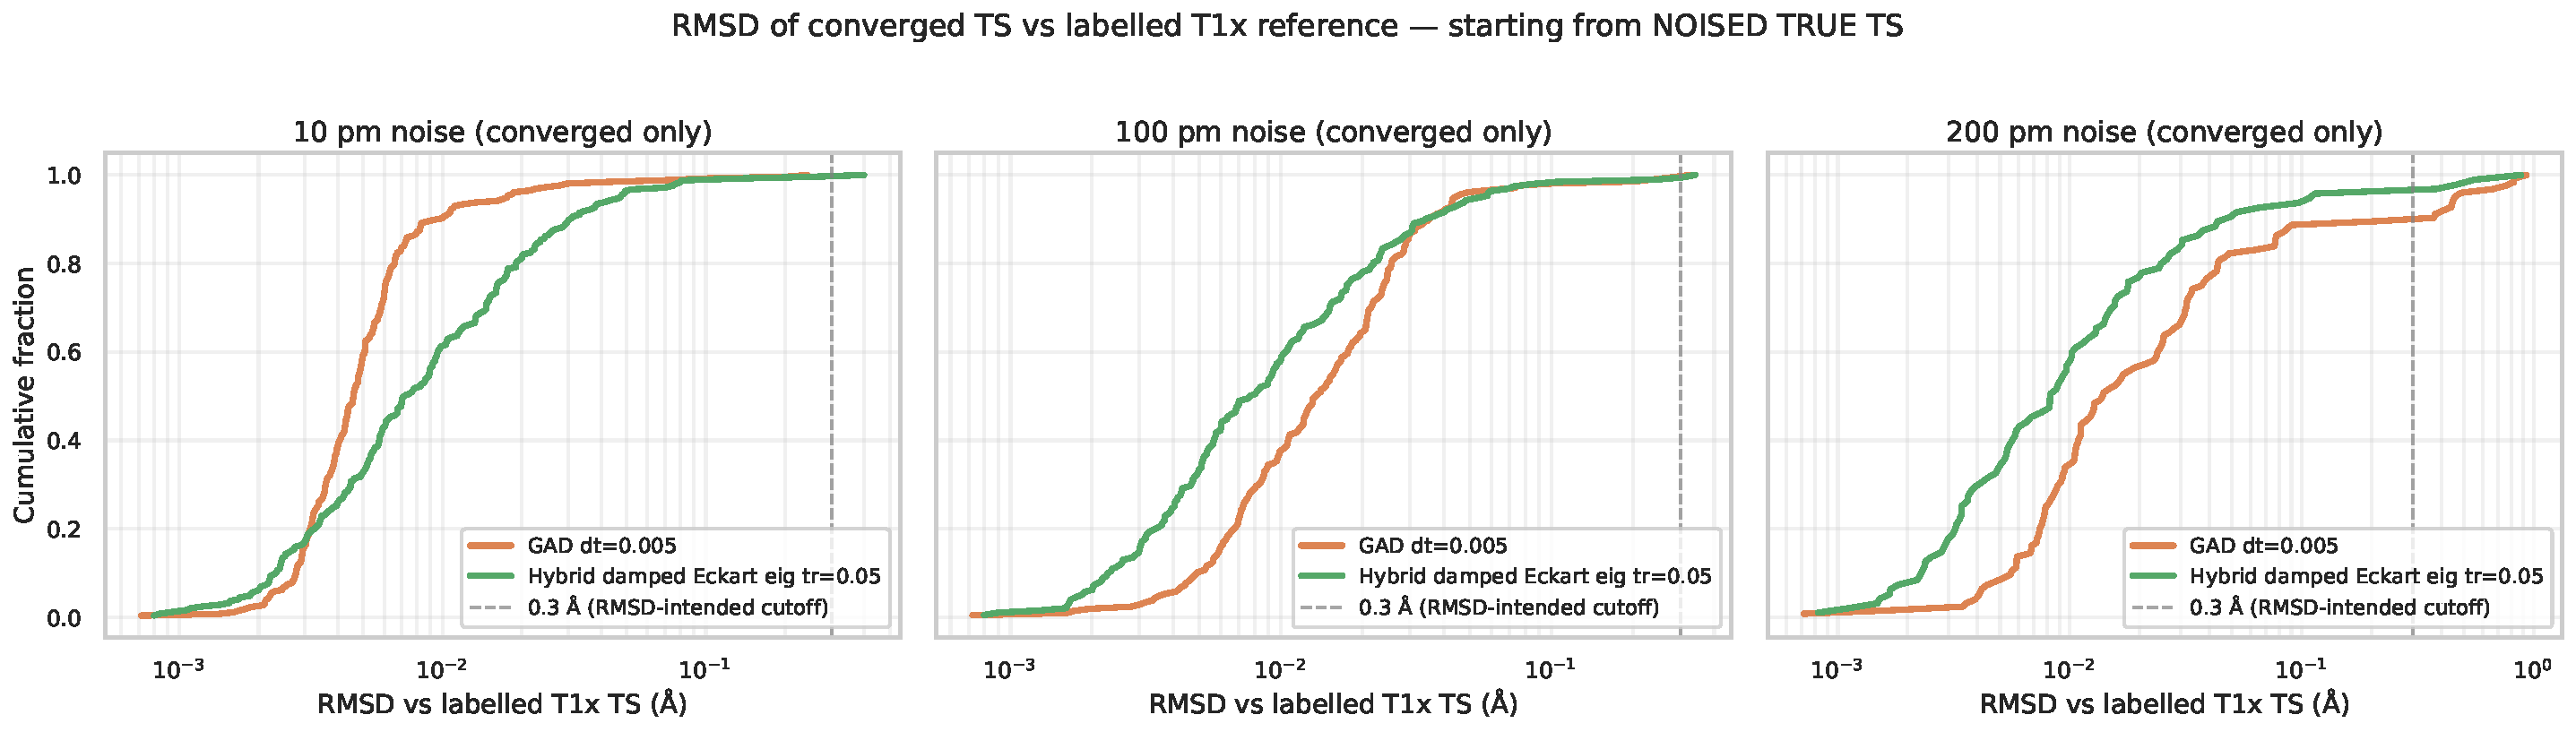
\includegraphics[width=\textwidth]{figures_2026_05_16/fig_rmsd_to_ts.pdf}
\caption{\textbf{RMSD distributions of converged TSs vs the labelled
T1x reference.} CDFs across three noise levels (converged samples only).
At 10 pm all three families are tight ($\le 0.05$ Å). At 100 pm Sella develops
a long right tail; hybrid stays tight. At \textbf{200 pm} the hybrid is
dramatically tighter — green curve rises sharply at low RMSD while Sella's
blue and GAD's orange extend past 0.5 Å. The 0.3 Å threshold (dashed) is the
RMSD-intended cutoff. Source: \texttt{rmsd\_distributions\_2026\_05\_11.csv}.}
\end{figure}

\clearpage
% =================================================================
\section{Sella Hess.Freq.=3 surprise: 96.5\% at 10 pm, but the chemistry doesn't follow}
% =================================================================

\texttt{Sella cartesian Eckart untuned Hess.Freq.=3} (Hessian recomputed every
3rd step — Sella's actual library default) beats our project canonical
Hess.Freq.=1 by +3.8 pp at 10 pm TS conv (96.5\% vs 92.7\%) at identical
total wall-time. Less Hessian information, better conv: surprising.

\begin{center}\small
\textbf{Sella d=1 vs d=3 (cart+Eckart, $F_\mathrm{max}<0.01$, $n=287$ each)}\\[0.4em]
\begin{tabular}{l|cccc}
\toprule
\textbf{noise} & \textbf{d=1 conv \%} & \textbf{d=3 conv \%} & $\Delta$ \textbf{(pp)} & \textbf{wall (s)} \\
\midrule
10 pm  & 92.7 & \textbf{96.5} & \textbf{+3.8} & 13.4 / 13.3 \\
30 pm  & 92.0 & \textbf{95.5} & \textbf{+3.5} & 14.6 / 13.9 \\
50 pm  & 88.2 & \textbf{92.0} & \textbf{+3.8} & 20.4 / 21.2 \\
100 pm & 70.7 & \textbf{72.8} & +2.1          & 46.1 / 50.5 \\
150 pm & \textbf{54.0} & 50.5 & $-3.5$        & 71.6 / 79.0 \\
200 pm & \textbf{27.2} & 23.3 & $-3.9$ & 107.0 / 115.4 \\
\bottomrule
\end{tabular}
\end{center}

\paragraph{Mechanism: same compute budget, more cautious steps.} d=3 takes
$3\times$ more steps per converged sample (123 vs 43) but each step is 22\%
cheaper (no Hessian recompute). Total wall is identical $\sim$13.3 s. The
3 BFGS-updated steps between full diagonalizations are smaller and smoother
$\to$ less mode-jitter $\to$ more samples landing at the strict
$F_\mathrm{max}<0.01$ threshold without overshooting.

\paragraph{IRC TOPO reverses the verdict: d=1 wins chemistry at every noise.}

\begin{center}\small
\begin{tabular}{l|cccc}
\toprule
\textbf{noise} & \textbf{d=1 raw / IRC} & \textbf{d=3 raw / IRC} & $\Delta$ \textbf{raw} & $\Delta$ \textbf{IRC} \\
\midrule
10 pm  & 92.7 / 89.2 & \textbf{96.5} / 88.5 & $+3.8$ & $-0.7$ \\
30 pm  & 92.0 / 89.2 & \textbf{95.5} / 88.9 & $+3.5$ & $-0.3$ \\
50 pm  & 88.2 / 87.5 & \textbf{92.0} / 87.1 & $+3.8$ & $-0.4$ \\
100 pm & 70.7 / \textbf{72.5} & 72.8 / 70.4 & $+2.1$ & $\mathbf{-2.1}$ \\
150 pm & \textbf{54.0} / \textbf{49.8} & 50.5 / 45.3 & $-3.5$ & $\mathbf{-4.5}$ \\
200 pm & \textbf{27.2} / \textbf{23.3} & 23.3 / 22.0 & $-3.9$ & $-1.3$ \\
\bottomrule
\end{tabular}
\end{center}

The IRC gap widens with noise from $-0.7$ pp at 10 pm to $-4.5$ pp at
150 pm, then narrows to $-1.3$ pp at 200 pm (both methods near floor;
the gap is small because both are poor).
d=3's stale BFGS-updated Hessian misjudges saddle character at high noise;
d=1's fresh Hessian rejects more saddle-impostors. Net: the project's d=1
choice is justified — the 96.5\% raw-conv "win" is a wrong-saddle false
positive that IRC catches.

\begin{figure}[H]
\centering
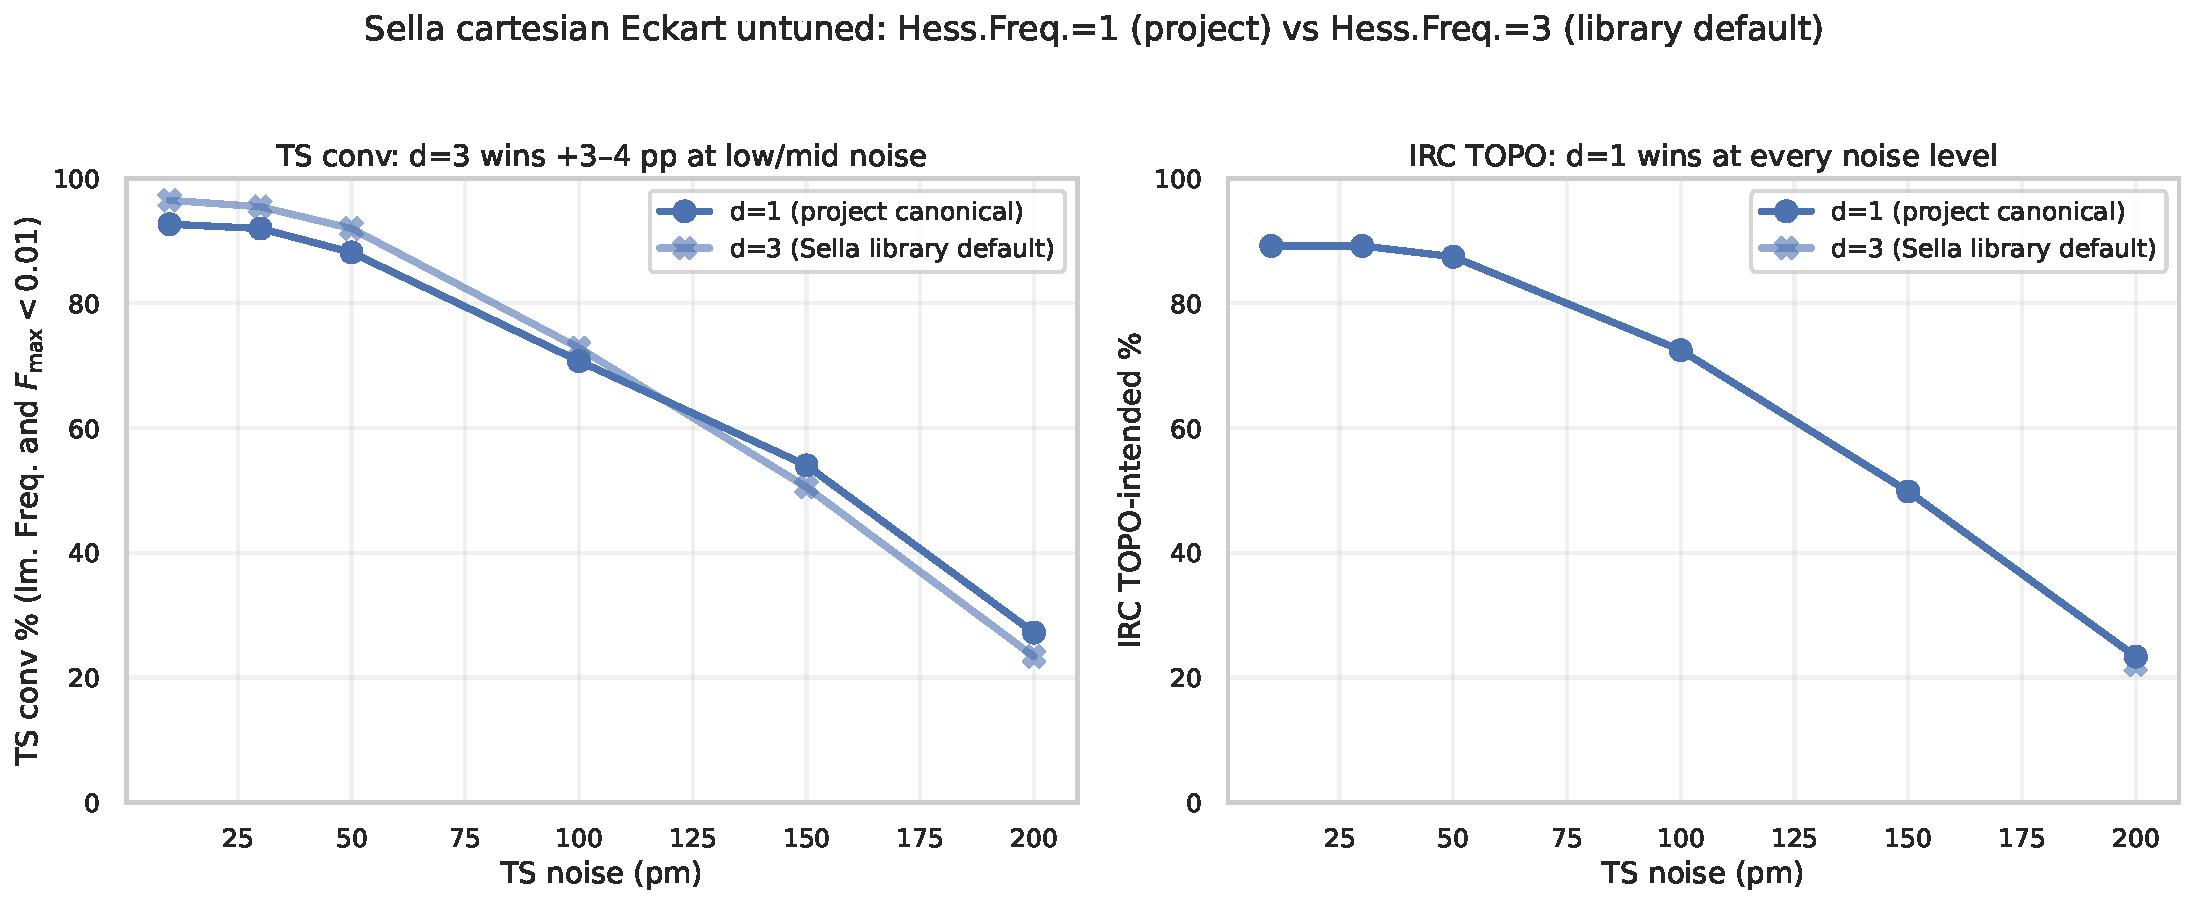
\includegraphics[width=\textwidth]{figures_2026_05_16/fig_d1_vs_d3.pdf}
\caption{\textbf{Sella cartesian Eckart untuned: Hess.Freq.=1 (project) vs
Hess.Freq.=3 (library default).} Left: d=3 wins TS conv +3--4 pp at low/mid
noise; loses at 150 pm. Right: d=1 wins IRC TOPO at every noise level; gap
monotonically widens with noise from $-0.7$ pp at 10 pm to $-4.5$ pp at
150 pm.}
\end{figure}

\clearpage
% =================================================================
\section{Newton-polish: can Newton break GAD's fmax plateau?}
% =================================================================

A direct test of the hybrid's ``other mode'' (the Newton-Raphson refinement
that fires when the GAD walk reaches $n_\mathrm{neg}=1$): can it crush
the force below the fmax plateau?

Two NR-GAD pingpong runs (SLURM 60314225, $n=80$, 50pm noise, 5000-step
budget) share identical dynamics (\texttt{nr\_max\_step\_norm=0.3},
\texttt{nr\_damping=1.0}) and differ only in the convergence target:

\begin{center}\small
\textbf{NR-GAD pingpong @ 50 pm noise, $n=80$.} Both runs use the same
spectral-partitioned NR + GAD flip-flop with trust-radius cap; only the
target threshold differs.\\[0.3em]
\begin{tabular}{l|cccc}
\toprule
\textbf{variant} & \textbf{$F_\mathrm{max}<0.05$} & \textbf{$F_\mathrm{max}<0.01$}
& \textbf{$F_\mathrm{max}<0.005$} & \textbf{$F_\mathrm{max}<0.001$} \\
\midrule
loose (stops at 0.01)            & 70.0 & 46.2 & 0.0  & 0.0 \\
\textbf{strict} (drives to 1e-4) & 73.8 & 45.0 & \textbf{31.2} & \textbf{1.2} \\
\midrule
\textit{baseline GAD dt=0.007 (2k steps)} & \textit{94.8} & \textit{85.7} & \textit{0.0} & \textit{0.0} \\
\bottomrule
\end{tabular}
\end{center}

Three observations:

\begin{itemize}[leftmargin=1.5em, itemsep=0.05em]
\item \textbf{Strict NR-polish DOES break the GAD plateau.}
  31.2\% reach $F_\mathrm{max}<0.005$ and 1.2\% reach $F_\mathrm{max}<0.001$
  on 50 pm noise. This is the only configuration tested on HIP/T1x that
  produces non-zero conversion at the Sella README threshold (0.001).
  The strict variant matches the same pattern across 50/100/150/200 pm
  noise: 1.2\% at 0.001 (i.e.\ 1 of 80 samples per noise level).
\item \textbf{The overshoot tax is real.} Trading away $\sim$40 pp of
  loose-threshold conversion (85.7\% $\to$ 45\%) buys $\sim$31 pp of
  tight-threshold conversion. Net: NR-polish redistributes successful
  conversions toward tighter geometries at the cost of looser conversions.
\item \textbf{Loose NR-polish gets the worst of both worlds:} it stops
  refining at 0.01 (no plateau-breaking) and pays the overshoot cost
  anyway (85.7\% $\to$ 46.2\%) because the NR phase fires before the
  loose criterion triggers exit. \emph{Loose is strictly dominated.}
\end{itemize}

\paragraph{Mechanism: trust radius is essential.} The pingpong's
\texttt{nr\_max\_step\_norm=0.3} caps each NR step at 0.3 Å, preventing
the $H^{-1}F$ blowup that occurs when an eigenvalue is near zero (close
to a saddle). Without the trust-radius cap, raw NR would overshoot
catastrophically — confirmed by the prior negative-result framing of the
``raw NR-polish'' attempt that did not break $F_\mathrm{max}<0.001$ for
any sample. The same conclusion applies to the long-budget probe
(hybrid damped @ 10k from noised TS): even with $5\times$ step budget,
no sample reached $F_\mathrm{max}<0.001$ on the partial $n=72$ data.

\paragraph{Why not just use this for the headline.} The strict
NR-polish trades 40 pp of loose conv for 31 pp of tight conv — the choice
depends on the use case. For a paper headline comparing TS finders at
the project-canonical $F_\mathrm{max}<0.01$ criterion, the hybrid damped
Eckart eig-switch tr=0.05 (which doesn't overshoot the plateau) is the
right reference. For a use case demanding sub-plateau geometric
precision (e.g.\ thermochemistry where strict TS optimization is
required), strict NR-polish is competitive with Sella's RFO and reaches
similar tight thresholds.

\paragraph{Sample sizes.} $n=80$ per cell (smaller than the
headline $n=287$). The 1.2\% at $F_\mathrm{max}<0.001$ corresponds to
$1/80$ samples per noise level — a real signal but not a precise rate.
Source: \texttt{runs/test\_nrpolish/nr\_gad\_polish\_dt007\_\{loose,strict\}/}.

\clearpage
% =================================================================
\section*{Open questions / future work}
% =================================================================

\begin{itemize}[leftmargin=1.5em, itemsep=0.1em]
\item \textbf{R1. Hess.Freq.=3 at 200 pm.} \textbf{DONE} (n=287 pooled, 23.3\%).
  d=3 vs d=1 raw conv gap: -3.9 pp. IRC TOPO @ 200 pm: 22.0\% (gap -1.3 pp).
\item \textbf{R2. Sella internal at 150 pm / 200 pm.} \textbf{DONE for 200 pm}
  (n=287 pooled, 13.9\%; IRC TOPO 16.0\%, +2.1 pp recovery). 150 pm refill
  in flight (SLURM 61166201).
\item \textbf{R3. Tighter $F_\mathrm{max}$ via longer step budget.} \textbf{DONE}.
  GAD ×10000 @ 50 pm produces \textbf{0\% conv at $F_\mathrm{max}<0.005$}
  on n=287 — confirms the plateau is structural, not budget-limited.
\item \textbf{R4. Mode-overlap-aware switching for hybrid.} Not started.
  Gate Newton trigger on eigenvector continuity in addition to
  $n_\mathrm{neg}{=}1$. Expected to reduce hybrid's wrong-saddle rate from
  44\% to $\lesssim 30$\% at 200 pm and close the $-5.9$ pp IRC TOPO gap vs
  plain GAD.
\end{itemize}

% =================================================================
\section{Sources \& reproducibility}\label{sec:sources}
% =================================================================

\begin{itemize}[leftmargin=1.5em, itemsep=0.05em]
\item \textbf{Master 4-axis table}: \texttt{analysis\_2026\_04\_29/master\_2026\_05\_11.csv}
\item \textbf{Threshold sweep table (5 thresholds $\times$ 9 methods $\times$ 6 noises)}: \texttt{analysis\_2026\_04\_29/threshold\_sweep\_2026\_05\_16.csv}
\item \textbf{Findings catalog}: \texttt{HYBRID\_FINDINGS\_CATALOG.md} (1180+ lines)
\item \textbf{Per-cell summaries}: \texttt{runs/hybrid\_for\_irc/}, \texttt{runs/hybrid\_deeper/}, \texttt{runs/hybrid\_extension/}, \texttt{runs/test\_dtgrid/}, \texttt{runs/test\_hessfreq/}, \texttt{runs/test\_reactant/}, \texttt{runs/starting\_geom\_300/}
\item \textbf{IRC validation parquets}: \texttt{runs/irc\_hybrid/}, \texttt{runs/irc\_hybrid\_deeper/}, \texttt{runs/irc\_hybrid\_extension/}, \texttt{runs/test\_irc/}, \texttt{runs/irc\_sella\_libdef\_d3/}
\item \textbf{Hybrid step functions}: \texttt{src/gadplus/search/hybrid\_gad\_damped\_eigfollownewton\_eckart.py}, \texttt{src/gadplus/search/hybrid\_gad\_eigfollownewton\_eckart.py}, \texttt{src/gadplus/search/hybrid\_gad\_eigfollownewton.py}
\item \textbf{Standalone runner}: \texttt{scripts/hybrid\_gad\_newton\_runner.py}
\item \textbf{Figure-build script}: \texttt{scripts/build\_pdf\_2026\_05\_16.py}
\end{itemize}

\paragraph{Partial-data caveat.} Cells marked with $^p$ in the headline tables
are extracted from SLURM logs after TIMEOUT and reflect $n<287$ samples — biased
toward smaller molecules (earlier sample\_ids). Full cells require resubmission
with longer wall-clock.

\end{document}
